\documentclass[9pt,hyperref={pdfpagemode=FullScreen,urlcolor=blue},xcolor=x11names]{beamer}

\mode<presentation>
{
  \usetheme{Warsaw}
  %\usetheme{Darmstadt}
  %\usetheme{Marburg}
  \setbeamertemplate{navigation symbols}{}

  %\usecolortheme{crane}
  %\usecolortheme{rose,sidebartab}

  \usecolortheme{beaver}
  %\usecolortheme{lily,sidebartab}
  %\usecolortheme{seahorse}

  \usefonttheme{serif}

  \setbeamertemplate{footline}[page number]
  \setbeamertemplate{sidebar canvas right}[vertical shading][top=palette
  primary.bg,%,middle=white,
  bottom=palette primary.bg]
  %\setbeamertemplate{sections/subsections in toc}[section numbered,subsection numbered]

  %\setbeamertemplate{itemize subitem}[circle]

  \setbeamercovered{transparent}

  %\beamertemplatenavigationsymbolsempty

  \useinnertheme{default}
}

\usepackage[utf8]{inputenc}
\usepackage[T1]{fontenc}
\usepackage{lmodern}
\usepackage{xspace}
\usepackage{amsmath,amssymb}
\usepackage[english]{babel}
%\usepackage[latin1]{inputenc}
%\usepackage[T1]{fontenc}
\usepackage{aeguill,fourier}

% souligne, barre
\usepackage{ulem}
%\usepackage[x11names]{xcolor}

\usepackage{pgf,pgfarrows,pgfnodes,pgfautomata,pgfheaps,pgfshade}


\usepackage{wasysym}
\usepackage{fancyvrb}
%\usepackage{verbatim}
\usepackage{marvosym}

\usepackage{colortbl}

\usepackage{pdftricks}
\begin{psinputs}
\usepackage{pstricks}
\usepackage{pst-bar}
\usepackage{pstricks-add}
\end{psinputs}

\usepackage{ulem}

\usepackage{ifdraft}
\usepackage{animate}
\usepackage{multimedia}

%\usepackage{texmath}

\usepackage{tikz}
\usetikzlibrary{calc}
\usetikzlibrary{patterns}   % for hatching
\usetikzlibrary{positioning}
\usetikzlibrary{decorations.pathreplacing}
\usetikzlibrary{decorations.pathmorphing}
\usetikzlibrary{arrows, decorations.markings}
\usetikzlibrary{shapes.geometric}
\newcommand{\warningsign}{\tikz[baseline=-.75ex] \node[shape=regular polygon, regular polygon sides=3, inner sep=0pt, draw, thick] {\textbf{!}};}
\newcommand{\reddanger}{\textcolor{red}{\danger}}


% the following is from 
% http://tex.stackexchange.com/questions/4811/make-first-row-of-table-all-bold
%\usepackage{array}
%\newcolumntype{$}{>{\global\let\currentrowstyle\relax}}
%\newcolumntype{^}{>{\currentrowstyle}}
%\newcommand{\rowstyle}[1]{\gdef\currentrowstyle{#1}%
%  #1\ignorespaces
%}

\usepackage{listings}
\usepackage{minted}

\usepackage{caption}


%%%%%%%%%%%%%%%%%%%
\hypersetup{%
  pdftitle={PATC-KOKKOS-2017},%
  pdfauthor={Pierre Kestener - CEA Saclay - MDLS - http://www.maisondelasimulation.fr},
  pdfsubject={Introdcution to Kokkos},
  pdfkeywords={KOKKOS, C++, GPU},
  pdfproducer={pdflatex avec la classe BEAMER},
  bookmarksopen=false,
  urlcolor=blue
}

%%%%%%%%%%%%%%%%%%%%%%%%%%%%%%%%%%%%%%%%%%%%%%%%%%%%%%%%%%%%%%%
%%%%%%%%%%%%%%%%%%%%%%%%%%%%%%%%%%%%%%%%%%%%%%%%%%%%%%%%%%%%%%%
%%%%%%%%%%%%%%%%%%%%%%%%%%%%%%%%%%%%%%%%%%%%%%%%%%%%%%%%%%%%%%%

\title{Kokkos, Modern C++, performance portability, ...}

\author
{
  \mbox{\underline{Pierre Kestener}}\inst{1}
}

\institute[mdls sap]{%
  \inst{1}%
  CEA Saclay, DSM, Maison de la Simulation
}

\date{PATC, January, 16-18th, 2017}

\pgfdeclareimage[height=0.5cm]{university-logo}{./images/Sigle-mdls}
\logo{\pgfuseimage{university-logo}}


%%%%%%%%%%%%%%%%%%%%%
\pgfdeclareimage[width=2.0cm]{sigle-cea}{./images/Sigle-mdls}
\pgfdeclareimage[width=2.0cm]{sigle-prace}{images/logo_prace}
\pgfdeclareimage[width=2.0cm]{sigle-nvidia}{images/NV_CUDA_Teaching_Center_3D.jpg}

\titlegraphic{
  % \pgfuseimage{sigle-prace}
  \hfill
  \pgfuseimage{sigle-cea}
  \hfill
  % \pgfuseimage{sigle-nvidia}
}



\begin{document}


\definecolor{green2}{rgb}{0.1,0.8,0.1} 
\definecolor{trust}{rgb}{0.71,0.14,0.07}
\definecolor{FancyPurple}{rgb}{0.5176, 0.1137, 0.2314}

\colorlet{redshaded}{red!25!bg}
\colorlet{shaded}{black!25!bg}
\colorlet{shadedshaded}{black!10!bg}
\colorlet{blackshaded}{black!40!bg}

\colorlet{darkred}{red!80!black}
\colorlet{darkblue}{blue!80!black}
\colorlet{darkgreen}{green!70!black}
\colorlet{greenshaded}{green!95!bg}
%\colorlet{coral}{Coral1!95!bg}

%red, green, blue, cyan, magenta, yellow, black, white, darkgray, gray,
%lightgray, brown, lime, olive, orange, pink, purple, teal, violet

\newcommand\myurl[1]{\textcolor{purple}{\underline{\url{#1}}}}
\newcommand\myhref[2]{\textcolor{purple}{\underline{\href{#1}{#2}}}}

\newcommand\mySmiley{\textcolor{darkgreen}{\Smiley{}}}
\newcommand\myFrowny{\textcolor{red}{\Frowny{}}}

%% Big-O notation.
\providecommand{\OO}[1]{\ensuremath{\operatorname{O}\bigl(#1\bigr)}}

% definition des couleurs pour affichage de code
\makeatletter
\def\PY@reset{\let\PY@it=\relax \let\PY@bf=\relax%
    \let\PY@ul=\relax \let\PY@tc=\relax%
    \let\PY@bc=\relax \let\PY@ff=\relax}
\def\PY@tok#1{\csname PY@tok@#1\endcsname}
\def\PY@toks#1+{\ifx\relax#1\empty\else%
    \PY@tok{#1}\expandafter\PY@toks\fi}
\def\PY@do#1{\PY@bc{\PY@tc{\PY@ul{%
    \PY@it{\PY@bf{\PY@ff{#1}}}}}}}
\def\PY#1#2{\PY@reset\PY@toks#1+\relax+\PY@do{#2}}

\def\PY@tok@gd{\def\PY@tc##1{\textcolor[rgb]{0.63,0.00,0.00}{##1}}}
\def\PY@tok@gu{\let\PY@bf=\textbf\def\PY@tc##1{\textcolor[rgb]{0.50,0.00,0.50}{##1}}}
\def\PY@tok@gt{\def\PY@tc##1{\textcolor[rgb]{0.00,0.25,0.82}{##1}}}
\def\PY@tok@gs{\let\PY@bf=\textbf}
\def\PY@tok@gr{\def\PY@tc##1{\textcolor[rgb]{1.00,0.00,0.00}{##1}}}
\def\PY@tok@cm{\let\PY@it=\textit\def\PY@tc##1{\textcolor[rgb]{0.25,0.50,0.50}{##1}}}
\def\PY@tok@vg{\def\PY@tc##1{\textcolor[rgb]{0.10,0.09,0.49}{##1}}}
\def\PY@tok@m{\def\PY@tc##1{\textcolor[rgb]{0.40,0.40,0.40}{##1}}}
\def\PY@tok@mh{\def\PY@tc##1{\textcolor[rgb]{0.40,0.40,0.40}{##1}}}
\def\PY@tok@go{\def\PY@tc##1{\textcolor[rgb]{0.50,0.50,0.50}{##1}}}
\def\PY@tok@ge{\let\PY@it=\textit}
\def\PY@tok@vc{\def\PY@tc##1{\textcolor[rgb]{0.10,0.09,0.49}{##1}}}
\def\PY@tok@il{\def\PY@tc##1{\textcolor[rgb]{0.40,0.40,0.40}{##1}}}
\def\PY@tok@cs{\let\PY@it=\textit\def\PY@tc##1{\textcolor[rgb]{0.25,0.50,0.50}{##1}}}
\def\PY@tok@cp{\def\PY@tc##1{\textcolor[rgb]{0.74,0.48,0.00}{##1}}}
\def\PY@tok@gi{\def\PY@tc##1{\textcolor[rgb]{0.00,0.63,0.00}{##1}}}
\def\PY@tok@gh{\let\PY@bf=\textbf\def\PY@tc##1{\textcolor[rgb]{0.00,0.00,0.50}{##1}}}
\def\PY@tok@ni{\let\PY@bf=\textbf\def\PY@tc##1{\textcolor[rgb]{0.60,0.60,0.60}{##1}}}
\def\PY@tok@nl{\def\PY@tc##1{\textcolor[rgb]{0.63,0.63,0.00}{##1}}}
\def\PY@tok@nn{\let\PY@bf=\textbf\def\PY@tc##1{\textcolor[rgb]{0.00,0.00,1.00}{##1}}}
\def\PY@tok@no{\def\PY@tc##1{\textcolor[rgb]{0.53,0.00,0.00}{##1}}}
\def\PY@tok@na{\def\PY@tc##1{\textcolor[rgb]{0.49,0.56,0.16}{##1}}}
\def\PY@tok@nb{\def\PY@tc##1{\textcolor[rgb]{0.00,0.50,0.00}{##1}}}
\def\PY@tok@nc{\let\PY@bf=\textbf\def\PY@tc##1{\textcolor[rgb]{0.00,0.00,1.00}{##1}}}
\def\PY@tok@nd{\def\PY@tc##1{\textcolor[rgb]{0.67,0.13,1.00}{##1}}}
\def\PY@tok@ne{\let\PY@bf=\textbf\def\PY@tc##1{\textcolor[rgb]{0.82,0.25,0.23}{##1}}}
\def\PY@tok@nf{\def\PY@tc##1{\textcolor[rgb]{0.00,0.00,1.00}{##1}}}
\def\PY@tok@si{\let\PY@bf=\textbf\def\PY@tc##1{\textcolor[rgb]{0.73,0.40,0.53}{##1}}}
\def\PY@tok@s2{\def\PY@tc##1{\textcolor[rgb]{0.73,0.13,0.13}{##1}}}
\def\PY@tok@vi{\def\PY@tc##1{\textcolor[rgb]{0.10,0.09,0.49}{##1}}}
\def\PY@tok@nt{\let\PY@bf=\textbf\def\PY@tc##1{\textcolor[rgb]{0.00,0.50,0.00}{##1}}}
\def\PY@tok@nv{\def\PY@tc##1{\textcolor[rgb]{0.10,0.09,0.49}{##1}}}
\def\PY@tok@s1{\def\PY@tc##1{\textcolor[rgb]{0.73,0.13,0.13}{##1}}}
\def\PY@tok@sh{\def\PY@tc##1{\textcolor[rgb]{0.73,0.13,0.13}{##1}}}
\def\PY@tok@sc{\def\PY@tc##1{\textcolor[rgb]{0.73,0.13,0.13}{##1}}}
\def\PY@tok@sx{\def\PY@tc##1{\textcolor[rgb]{0.00,0.50,0.00}{##1}}}
\def\PY@tok@bp{\def\PY@tc##1{\textcolor[rgb]{0.00,0.50,0.00}{##1}}}
\def\PY@tok@c1{\let\PY@it=\textit\def\PY@tc##1{\textcolor[rgb]{0.25,0.50,0.50}{##1}}}
\def\PY@tok@kc{\let\PY@bf=\textbf\def\PY@tc##1{\textcolor[rgb]{0.00,0.50,0.00}{##1}}}
\def\PY@tok@c{\let\PY@it=\textit\def\PY@tc##1{\textcolor[rgb]{0.25,0.50,0.50}{##1}}}
\def\PY@tok@mf{\def\PY@tc##1{\textcolor[rgb]{0.40,0.40,0.40}{##1}}}
\def\PY@tok@err{\def\PY@bc##1{\fcolorbox[rgb]{1.00,0.00,0.00}{1,1,1}{##1}}}
\def\PY@tok@kd{\let\PY@bf=\textbf\def\PY@tc##1{\textcolor[rgb]{0.00,0.50,0.00}{##1}}}
\def\PY@tok@ss{\def\PY@tc##1{\textcolor[rgb]{0.10,0.09,0.49}{##1}}}
\def\PY@tok@sr{\def\PY@tc##1{\textcolor[rgb]{0.73,0.40,0.53}{##1}}}
\def\PY@tok@mo{\def\PY@tc##1{\textcolor[rgb]{0.40,0.40,0.40}{##1}}}
\def\PY@tok@kn{\let\PY@bf=\textbf\def\PY@tc##1{\textcolor[rgb]{0.00,0.50,0.00}{##1}}}
\def\PY@tok@mi{\def\PY@tc##1{\textcolor[rgb]{0.40,0.40,0.40}{##1}}}
\def\PY@tok@gp{\let\PY@bf=\textbf\def\PY@tc##1{\textcolor[rgb]{0.00,0.00,0.50}{##1}}}
\def\PY@tok@o{\def\PY@tc##1{\textcolor[rgb]{0.40,0.40,0.40}{##1}}}
\def\PY@tok@kr{\let\PY@bf=\textbf\def\PY@tc##1{\textcolor[rgb]{0.00,0.50,0.00}{##1}}}
\def\PY@tok@s{\def\PY@tc##1{\textcolor[rgb]{0.73,0.13,0.13}{##1}}}
\def\PY@tok@kp{\def\PY@tc##1{\textcolor[rgb]{0.00,0.50,0.00}{##1}}}
\def\PY@tok@w{\def\PY@tc##1{\textcolor[rgb]{0.73,0.73,0.73}{##1}}}
\def\PY@tok@kt{\def\PY@tc##1{\textcolor[rgb]{0.69,0.00,0.25}{##1}}}
\def\PY@tok@ow{\let\PY@bf=\textbf\def\PY@tc##1{\textcolor[rgb]{0.67,0.13,1.00}{##1}}}
\def\PY@tok@sb{\def\PY@tc##1{\textcolor[rgb]{0.73,0.13,0.13}{##1}}}
\def\PY@tok@k{\let\PY@bf=\textbf\def\PY@tc##1{\textcolor[rgb]{0.00,0.50,0.00}{##1}}}
\def\PY@tok@se{\let\PY@bf=\textbf\def\PY@tc##1{\textcolor[rgb]{0.73,0.40,0.13}{##1}}}
\def\PY@tok@sd{\let\PY@it=\textit\def\PY@tc##1{\textcolor[rgb]{0.73,0.13,0.13}{##1}}}

\def\PYZbs{\char`\\}
\def\PYZus{\char`\_}
\def\PYZob{\char`\{}
\def\PYZcb{\char`\}}
\def\PYZca{\char`\^}
\def\PYZsh{\char`\#}
\def\PYZpc{\char`\%}
\def\PYZdl{\char`\$}
\def\PYZti{\char`\~}

\newcommand\lb{[}
\newcommand\rb{]}
\newcommand\PYbg[1]{\textcolor[rgb]{0.00,0.50,0.00}{\textbf{#1}}}
\newcommand\PYbf[1]{\textcolor[rgb]{0.73,0.40,0.53}{\textbf{#1}}}
\newcommand\PYbe[1]{\textcolor[rgb]{0.40,0.40,0.40}{#1}}
\newcommand\PYbd[1]{\textcolor[rgb]{0.73,0.13,0.13}{#1}}
\newcommand\PYbc[1]{\textcolor[rgb]{0.00,0.50,0.00}{\textbf{#1}}}
\newcommand\PYbb[1]{\textcolor[rgb]{0.40,0.40,0.40}{#1}}
\newcommand\PYba[1]{\textcolor[rgb]{0.00,0.00,0.50}{\textbf{#1}}}
\newcommand\PYaJ[1]{\textcolor[rgb]{0.73,0.13,0.13}{#1}}
\newcommand\PYaK[1]{\textcolor[rgb]{0.00,0.00,1.00}{#1}}
\newcommand\PYaH[1]{\fcolorbox[rgb]{1.00,0.00,0.00}{1,1,1}{#1}}
\newcommand\PYaI[1]{\textcolor[rgb]{0.69,0.00,0.25}{#1}}
\newcommand\PYaN[1]{\textcolor[rgb]{0.00,0.00,1.00}{\textbf{#1}}}
\newcommand\PYaO[1]{\textcolor[rgb]{0.00,0.00,0.50}{\textbf{#1}}}
\newcommand\PYaL[1]{\textcolor[rgb]{0.73,0.73,0.73}{#1}}
\newcommand\PYaM[1]{\textcolor[rgb]{0.74,0.48,0.00}{#1}}
\newcommand\PYaB[1]{\textcolor[rgb]{0.00,0.25,0.82}{#1}}
\newcommand\PYaC[1]{\textcolor[rgb]{0.67,0.13,1.00}{#1}}
\newcommand\PYaA[1]{\textcolor[rgb]{0.00,0.50,0.00}{#1}}
\newcommand\PYaF[1]{\textcolor[rgb]{1.00,0.00,0.00}{#1}}
\newcommand\PYaG[1]{\textcolor[rgb]{0.10,0.09,0.49}{#1}}
\newcommand\PYaD[1]{\textcolor[rgb]{0.25,0.50,0.50}{\textit{#1}}}
\newcommand\PYaE[1]{\textcolor[rgb]{0.63,0.00,0.00}{#1}}
\newcommand\PYaZ[1]{\textcolor[rgb]{0.00,0.50,0.00}{\textbf{#1}}}
\newcommand\PYaX[1]{\textcolor[rgb]{0.00,0.50,0.00}{#1}}
\newcommand\PYaY[1]{\textcolor[rgb]{0.73,0.13,0.13}{#1}}
\newcommand\PYaR[1]{\textcolor[rgb]{0.10,0.09,0.49}{#1}}
\newcommand\PYaS[1]{\textcolor[rgb]{0.25,0.50,0.50}{\textit{#1}}}
\newcommand\PYaP[1]{\textcolor[rgb]{0.49,0.56,0.16}{#1}}
\newcommand\PYaQ[1]{\textcolor[rgb]{0.40,0.40,0.40}{#1}}
\newcommand\PYaV[1]{\textcolor[rgb]{0.00,0.00,1.00}{\textbf{#1}}}
\newcommand\PYaW[1]{\textcolor[rgb]{0.73,0.13,0.13}{#1}}
\newcommand\PYaT[1]{\textcolor[rgb]{0.50,0.00,0.50}{\textbf{#1}}}
\newcommand\PYaU[1]{\textcolor[rgb]{0.82,0.25,0.23}{\textbf{#1}}}
\newcommand\PYaj[1]{\textcolor[rgb]{0.00,0.50,0.00}{#1}}
\newcommand\PYak[1]{\textcolor[rgb]{0.73,0.40,0.53}{#1}}
\newcommand\PYah[1]{\textcolor[rgb]{0.63,0.63,0.00}{#1}}
\newcommand\PYai[1]{\textcolor[rgb]{0.10,0.09,0.49}{#1}}
\newcommand\PYan[1]{\textcolor[rgb]{0.67,0.13,1.00}{\textbf{#1}}}
\newcommand\PYao[1]{\textcolor[rgb]{0.73,0.40,0.13}{\textbf{#1}}}
\newcommand\PYal[1]{\textcolor[rgb]{0.25,0.50,0.50}{\textit{#1}}}
\newcommand\PYam[1]{\textbf{#1}}
\newcommand\PYab[1]{\textit{#1}}
\newcommand\PYac[1]{\textcolor[rgb]{0.73,0.13,0.13}{#1}}
\newcommand\PYaa[1]{\textcolor[rgb]{0.50,0.50,0.50}{#1}}
\newcommand\PYaf[1]{\textcolor[rgb]{0.25,0.50,0.50}{\textit{#1}}}
\newcommand\PYag[1]{\textcolor[rgb]{0.40,0.40,0.40}{#1}}
\newcommand\PYad[1]{\textcolor[rgb]{0.73,0.13,0.13}{#1}}
\newcommand\PYae[1]{\textcolor[rgb]{0.40,0.40,0.40}{#1}}
\newcommand\PYaz[1]{\textcolor[rgb]{0.00,0.63,0.00}{#1}}
\newcommand\PYax[1]{\textcolor[rgb]{0.60,0.60,0.60}{\textbf{#1}}}
\newcommand\PYay[1]{\textcolor[rgb]{0.00,0.50,0.00}{\textbf{#1}}}
\newcommand\PYar[1]{\textcolor[rgb]{0.10,0.09,0.49}{#1}}
\newcommand\PYas[1]{\textcolor[rgb]{0.73,0.13,0.13}{\textit{#1}}}
\newcommand\PYap[1]{\textcolor[rgb]{0.00,0.50,0.00}{#1}}
\newcommand\PYaq[1]{\textcolor[rgb]{0.53,0.00,0.00}{#1}}
\newcommand\PYav[1]{\textcolor[rgb]{0.00,0.50,0.00}{\textbf{#1}}}
\newcommand\PYaw[1]{\textcolor[rgb]{0.40,0.40,0.40}{#1}}
\newcommand\PYat[1]{\textcolor[rgb]{0.10,0.09,0.49}{#1}}
\newcommand\PYau[1]{\textcolor[rgb]{0.40,0.40,0.40}{#1}}


% for compatibility with earlier versions
\def\PYZat{@}
\def\PYZlb{[}
\def\PYZrb{]}
\makeatother



%%%%%%%%%%%%%%%%%%%%%
% 1ere page
\begin{frame}[label=courant]
  \titlepage
\end{frame}

%%%%%%%%%%%%%%%%%%%%%%%%%%%%%%%%%%%%%%%%%%%%%%%%%%%%%%%%%%%%%%%%%%%%%%%% 
%%%%%%%%%%%%%%%%%%%%%%%%%%%%%%%%%%%%%%%%%%%%%%%%%%%%%%%%%%%%%%%%%%%%%%%% 
\begin{frame}
  \frametitle{Schedule}

  {\bf \large \textcolor{violet}{Thrusday, May 31st, 2018:}} \textcolor{orange}{\bf Kokkos tutorial}
  \begin{itemize}
  \item GPU Computing / Cuda refresh % ~ 30 minutes
  \item \textcolor{red}{\bf Introduction performance portability} % ~ 30 minutes
  \item IBM Power8 + Nvidia Pascal P100 platform : short overview % ~ 30 minutes
  \item \textbf{C++ Kokkos: features overview} % ~ 30 minutes
  \item \textcolor{blue}{Hands-on 0:} \textbf{retrieve Kokkos sources}, how to build, how to run a \textit{helloworld} application, explore different configurations % ~ 40 minutes
  \item \textcolor{blue}{Hands-on 1:} cross-checking \textbf{Kokkos + hwloc} is OK
  \item \textbf{Replay some tutorial slides from SC2016 for deeper Kokkos concepts}
  \item \textcolor{blue}{Hands-On 2:} Simple example \textbf{SAXPY}\\
    \textcolor{darkgreen}{$\Rightarrow$ simplest computing kernel in Kokkos} % ~ 45 minutes
  \item \textcolor{blue}{Hands-On 3:} Simple example \textbf{Mandelbrot set}\\
    \textcolor{darkgreen}{$\Rightarrow$ 1D Kokkos::View + linearized index (+ asynchronous execution)} % ~ 30 mintes
  \item {\bf a Kokkos miniapp skeleton project with cmake} 
  \end{itemize}
\end{frame}

%%%%%%%%%%%%%%%%%%%%%%%%%%%%%%%%%%%%%%%%%%%%%%%%%%%%%%%%%%%%%%%%%%%%%%%% 
%%%%%%%%%%%%%%%%%%%%%%%%%%%%%%%%%%%%%%%%%%%%%%%%%%%%%%%%%%%%%%%%%%%%%%%% 
\begin{frame}
  \frametitle{Schedule}

  {\bf \large \textcolor{violet}{Friday, June 1st, 2018:}} \textcolor{orange}{\bf Kokkos tutorial}
  \begin{itemize}
  \item \textcolor{blue}{Hands-On 4:} Simple examples \textbf{Stencil + Finite Difference}\\
    \textcolor{darkgreen}{$\Rightarrow$ 2D Kokkos::View}
  \item \textcolor{blue}{Hands-On 5:} \textbf{Laplace exercice}\\
    \textcolor{darkgreen}{$\Rightarrow$ pure Kokkos versus Kokkos + MPI + hwloc (multiGPU)}
  \item \textcolor{blue}{Hands-On 6:} \textbf{Illustrate how to use random number generator in kokkos}\\
    \textcolor{darkgreen}{$\Rightarrow$ RNG 101, parallel compute $\pi$ with Monte Carlo}
  \item \textcolor{blue}{Hands-On 7:} CSCS miniApp: \textbf{Fisher equation solver}\\
    \textcolor{darkgreen}{$\Rightarrow$ use Kokkos lambda}
  \item \textcolor{blue}{Hands-On 8:} CFD miniApp: \textbf{Euler solver}\\
    \textcolor{darkgreen}{$\Rightarrow$ performance measurement for several Kokkos backends (OpenMP, CUDA)}
  \end{itemize}
\end{frame}


\section{Introduction - Kokkos concepts}
%%%%%%%%%%%%%%%%%%%%%%%%%%%%%%%%%%%%%%%%%%%%%%%%%%%%%%%%%%%%%%%%%%% 
%%%%%%%%%%%%%%%%%%%%%%%%%%%%%%%%%%%%%%%%%%%%%%%%%%%%%%%%%%%%%%%%%%% 
%%%%%%%%%%%%%%%%%%%%%%%%%%%%%%%%%%%%%%%%%%%%%%%%%%%%%%%%%%%%%%%%%%% 
\begin{frame}
  \frametitle{Kokkos: a programming model for performance portability}

  \only<1>{
    \begin{itemize}
    \item \textcolor{blue}{\textbf{Kokkos}} is a \textbf{C++ library} with \textcolor{red}{\textbf{parallel algorithmic patterns}} AND \textcolor{red}{\textbf{data containers}} for \textcolor{blue}{\textbf{node-level parallelism}}.
    \item Implementation relies heavily on \textbf{meta-programing} to derive native {\bf low-level code (OpenMP, Pthreads, CUDA, ...)} and adapt data structure {\bf memory layout} at compile-time
    \item Core developers at \textcolor{violet}{\bf SANDIA NL} (\textbf{H.C. Edwards, C. Trott})
    \end{itemize}
  }
  \only<2>{
    \begin{itemize}
    \item \textcolor{darkgreen}{\textbf{Open source}}, \myurl{https://github.com/kokkos/kokkos}
    \item Primarily developped as a base building layer for \textbf{generic high-performance parallel linear algebra} in \myhref{https://github.com/trilinos/Trilinos}{Trilinos}
    \item Also used in molecular dynamics code, e.g. \myhref{http://lammps.sandia.gov/}{LAMMPS}
    \item Goal: \textcolor{orange}{\textbf{ISO/C++ 2020 Standard}} subsumes Kokkos abstractions~\footnote{see mdspan proposal \myurl{https://github.com/kokkos/array_ref}}
    \end{itemize}
  }
  \begin{center}
    \includegraphics<1-2>[width=7cm]{doc/perf_portability/kokkos_summary}
  \end{center}

\end{frame}

%%%%%%%%%%%%%%%%%%%%%%%%%%%%%%%%%%%%%%%%%%%%%%%%%%%%%%%%%%%%%%%%%%% 
%%%%%%%%%%%%%%%%%%%%%%%%%%%%%%%%%%%%%%%%%%%%%%%%%%%%%%%%%%%%%%%%%%% 
%%%%%%%%%%%%%%%%%%%%%%%%%%%%%%%%%%%%%%%%%%%%%%%%%%%%%%%%%%%%%%%%%%% 
\begin{frame}
  \frametitle{Kokkos: a programming model for performance portability}

  \begin{center}
    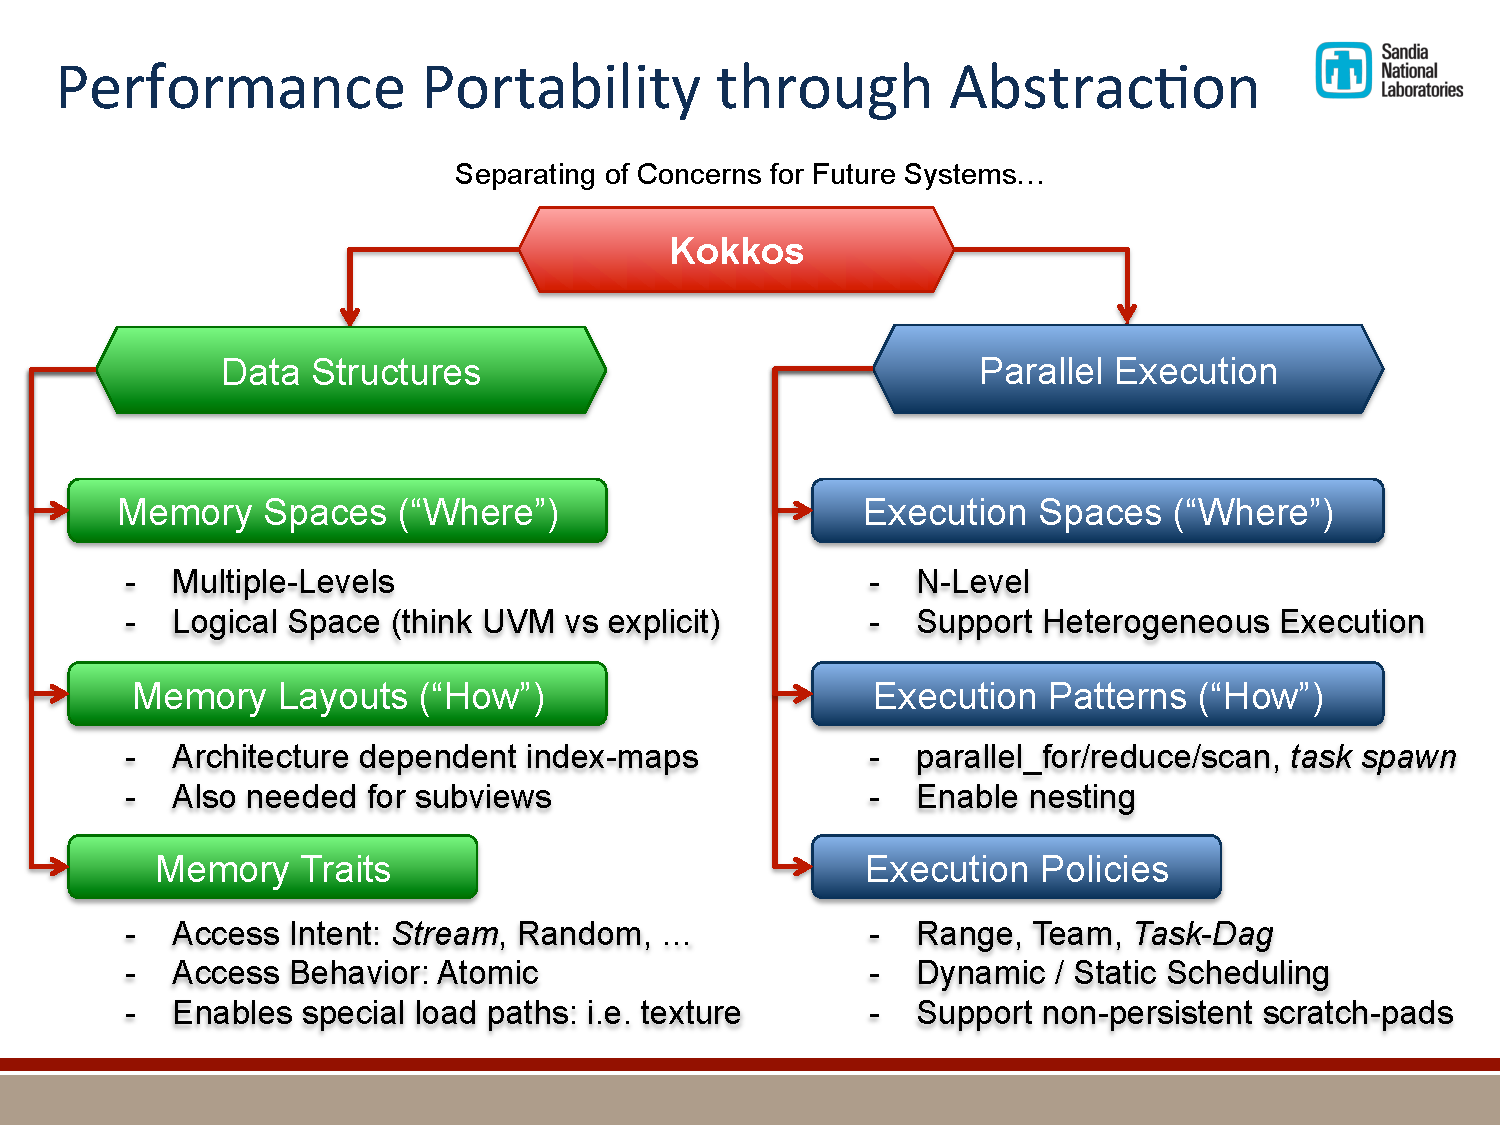
\includegraphics[width=8.0cm]{../intro/images/Kokkos-Multi-CoE_slide3}
  \end{center}

  {\small reference: \myurl{https://cfwebprod.sandia.gov/cfdocs/CompResearch/docs/Kokkos-Multi-CoE.pdf}}

\end{frame}


%%%%%%%%%%%%%%%%%%%%%%%%%%%%%%%%%%%%%%%%%%%%%%%%%%%%%%%%%%%%%%%%%%% 
%%%%%%%%%%%%%%%%%%%%%%%%%%%%%%%%%%%%%%%%%%%%%%%%%%%%%%%%%%%%%%%%%%% 
%%%%%%%%%%%%%%%%%%%%%%%%%%%%%%%%%%%%%%%%%%%%%%%%%%%%%%%%%%%%%%%%%%% 
\begin{frame}
  \frametitle{Kokkos Concepts (1) - the abstract machine model}

  \begin{itemize}
  \item Kokkos defines an abstract machine model for future large shared-memory nodes made of 
    \begin{itemize}
    \item \textcolor{blue}{\textbf{latency-oriented cores}} (contemporary CPU core)
    \item \textcolor{orange}{\textbf{throughput-oriented cores}} (GPU, ...)
    \end{itemize}
  \end{itemize}

  \begin{center}
    \begin{figure}
      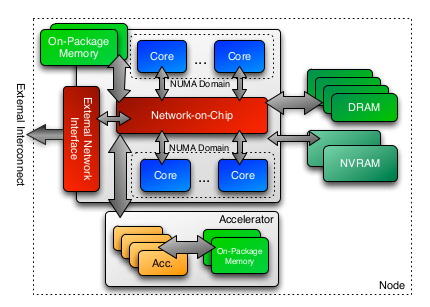
\includegraphics[width=5cm]{images/kokkos_machine_model}
      \caption{Conceptual model of a future HPC node. (Kokkos User's Guide).}
      \end{figure}
  \end{center}

\end{frame}


%%%%%%%%%%%%%%%%%%%%%%%%%%%%%%%%%%%%%%%%%%%%%%%%%%%%%%%%%%%%%%%%%%% 
%%%%%%%%%%%%%%%%%%%%%%%%%%%%%%%%%%%%%%%%%%%%%%%%%%%%%%%%%%%%%%%%%%% 
%%%%%%%%%%%%%%%%%%%%%%%%%%%%%%%%%%%%%%%%%%%%%%%%%%%%%%%%%%%%%%%%%%% 
\begin{frame}[fragile=singleslide]
  \frametitle{Kokkos Concepts (2) - What is a device ?}

  \begin{itemize}
  \item A \textcolor{red}{\textbf{Kokkos device}}: 
  \item From a C++ API design point of view, Kokkos defines several c++ class for a \textcolor{red}{device} in \texttt{core/src}, e.g.
    \begin{itemize}
    \item Kokkos::Cuda, Kokkos::OpenMP, Kokkos::Pthreads, Kokkos::Serial
    \item \textcolor{blue}{\textit{device} = execution space + memory space}
    \end{itemize}
  \item Each \textit{Kokkos device} pre-defines some types
  \item Example \textcolor{red}{\textbf{Kokkos device}} (not required for a user, only Kokkos developper), e.g.\\
    {\tiny
      \begin{minted}{c++}
        class Cuda {
          public:
          // Tag this class as a kokkos execution space
          typedef Cuda                  execution_space ;
          
          #if defined( KOKKOS_USE_CUDA_UVM )
          // This execution space's preferred memory space.
          typedef CudaUVMSpace          memory_space ;
          #else
          // This execution space's preferred memory space.
          typedef CudaSpace             memory_space ;
          #endif
          
          // This execution space preferred device_type
          typedef Kokkos::Device<execution_space,memory_space> device_type;
          
          // The size_type best suited for this execution space.
          typedef memory_space::size_type  size_type ;
          
          // This execution space's preferred array layout.
          typedef LayoutLeft            array_layout ;
          ...
        } // end class Cuda
        \end{minted}
      }
  \end{itemize}

\end{frame}

%%%%%%%%%%%%%%%%%%%%%%%%%%%%%%%%%%%%%%%%%%%%%%%%%%%%%%%%%%%%%%%%%%% 
%%%%%%%%%%%%%%%%%%%%%%%%%%%%%%%%%%%%%%%%%%%%%%%%%%%%%%%%%%%%%%%%%%% 
%%%%%%%%%%%%%%%%%%%%%%%%%%%%%%%%%%%%%%%%%%%%%%%%%%%%%%%%%%%%%%%%%%% 
\begin{frame}
  \frametitle{Kokkos Concepts (3) - execution space, memory space}

  \begin{itemize}
  \item \textcolor{blue}{\textbf{Execution space:}} Where should a parallel contruct (\texttt{parallel\_for}, \texttt{parallel\_reduce}, ...) be executed\\
    \begin{itemize}
    \item Special case: \texttt{class HostSpace}, special device (always defined) where execution space is either (Serial, Pthread or OpenMP).
    \item Each execution space is equipped with a \texttt{fence}: \texttt{Kokkos::Cuda::fence()}
    \end{itemize}
  \item \textcolor{blue}{\textbf{Memory space:}} Where / how data are allocated in memory (HostSpace, CudaSpace, CudaUVMSpace, CudaHostPinnedSpace, HBWSpace, ...)
  \item \textcolor{blue}{\textbf{Memory layout}} (come back later on that)
  \item Other concepts:
    \begin{itemize}
    \item Execution policy: used to modify a parallel thread dispatch
    \end{itemize}
  \item \textcolor{red}{Multiple execution / memory space} can be used in a single application\\
    See for example in Kokkos sources \texttt{example/tutorial/Advanced\_View/07\_Overlapping\_DeepCopy}\\
    Though, take care that currently, Cuda stream are completely mapped into Kokkos API~\footnote{Will be implemented in the coming months}; meanwhile Cuda streams can be used directly (but looses portability); 
  \end{itemize}

\end{frame}



\subsection{Build Kokkos}
%%%%%%%%%%%%%%%%%%%%%%%%%%%%%%%%%%%%%%%%%%%%%%%%%%%%%%%%%%%%%%%%%%%%%%%% 
%%%%%%%%%%%%%%%%%%%%%%%%%%%%%%%%%%%%%%%%%%%%%%%%%%%%%%%%%%%%%%%%%%%%%%%% 
\begin{frame}
  \frametitle{Hands-On 0: Build kokkos (1)}
  
  \textbf{0. Kokkos is still experimental, but moving fast: use git sources}
  
  \textbf{1. Get Kokkos sources, development branch - don't try to build yet !}
  \begin{itemize}
  \item \textcolor{blue}{Practicals on \texttt{ouessant}:}\\
    \textcolor{darkgreen}{\texttt{1. mkdir \$HOME/kokkos-tutorial; cd \$HOME/kokkos-tutorial}}\\
    some kokkos tutorial examples have a Makefile configured for using that precise location.\\
    \textcolor{darkgreen}{\texttt{2. git clone https://github.com/kokkos/kokkos}}\\
    \textcolor{darkgreen}{\texttt{3. cd kokkos; git checkout develop}}
  \end{itemize}
  
\end{frame}

%%%%%%%%%%%%%%%%%%%%%%%%%%%%%%%%%%%%%%%%%%%%%%%%%%%%%%%%%%%%%%%%%%%%%%%% 
%%%%%%%%%%%%%%%%%%%%%%%%%%%%%%%%%%%%%%%%%%%%%%%%%%%%%%%%%%%%%%%%%%%%%%%% 
\begin{frame}
  \frametitle{Hands-On 0: Build kokkos (2)}

  \textbf{2. How to build and use}
  \begin{enumerate}
  \item \textcolor{red}{\textbf{As a regular library (standalone Makefile, installed library):}} \\
    \begin{itemize}
    \item {\bf not recommended} for production level (see below), {\bf OK for testing and building examples}
    \item use \texttt{generate\_makefile.bash}, then \texttt{make kokkoslib; make install}\\
      Then use a \textit{modulefile} to configure the environment\\
      Kokkos examples (inside source) can be built that way, as well as \myhref{https://github.com/kokkos/kokkos-tutorials}{Kokkos-tutorials}
    \end{itemize}
  \item \textcolor{blue}{\textbf{Embedded Kokkos source files in your application}}
    \begin{itemize}
    \item Why ?
    \item $\Rightarrow$ Kokkos by design has {\bf many different configurations possible} (hardware adaptability, heavily relies on C++ metaprograming - compile timing )
    \item $\Rightarrow$ best practice advice : better compile kokkos as part as the target application (same flags, same compiler, etc...)
    \item $\Rightarrow$ \textcolor{blue}{\bf recommended use}:
    \textcolor{darkgreen}{\bf standalone \myhref{https://cmake.org/}{cmake} + kokkos sources embedded in your application} (we'll see a skeleton app)
    \end{itemize}
  \item There exists another cmake-based build sytem, but relies on a third-party tools \myhref{https://tribits.org/}{TriBITS}. Right now this can only be used used when Kokkos is build inside \myhref{https://github.com/trilinos/Trilinos}{Trilinos} (heterogeneous distributed sparse and dense linear algebra package).
  \end{enumerate}
 
\end{frame}

%%%%%%%%%%%%%%%%%%%%%%%%%%%%%%%%%%%%%%%%%%%%%%%%%%%%%%%%%%%%%%%%%%%%%%%% 
%%%%%%%%%%%%%%%%%%%%%%%%%%%%%%%%%%%%%%%%%%%%%%%%%%%%%%%%%%%%%%%%%%%%%%%% 
\begin{frame}
  \frametitle{Hands-On 0: Build kokkos (3)}

  {\bf \textcolor{red}{About standalone Makefile} and environment variables settings for building on multiple architectures}

  \begin{itemize}
  \item The following variables are usefull when building some of the tutorial examples :
    \begin{itemize}
    \item \texttt{KOKKOS\_PATH}: path to Kokkos source dir
    \item \texttt{KOKKOS\_DEVICES}: define possible execution spaces: CUDA, OpenMP, Pthreads, Serial, ...
    \item \texttt{KOKKOS\_ARCH}: used to customize compiler flags; e.g. Power8, Kepler35, SNB, KNL, ARMv80, ROCm, ...
    \end{itemize}
  \item When building for \textcolor{darkgreen}{\bf CUDA device}, you'll need to use Kokkos' own compiler wrapper: \textcolor{darkgreen}{\texttt{\bf nvcc\_wrapper}} (included in Kokkos sources), not just \texttt{nvcc}
  \item \textcolor{red}{When building Kokkos and aiming at an installed Kokkos}, the same information (in a different form) is passed to script \texttt{generate\_makefile.bash}\\
    Just type \texttt{./generate\_makefile.bash \--\--help} at top-level Kokkos sources
  \item \textcolor{blue}{When using Kokkos embedded in your application}, these variables must be set on the \texttt{make} command line.
  \end{itemize}
  
\end{frame}
  
%%%%%%%%%%%%%%%%%%%%%%%%%%%%%%%%%%%%%%%%%%%%%%%%%%%%%%%%%%%%%%%%%%%%%%%% 
%%%%%%%%%%%%%%%%%%%%%%%%%%%%%%%%%%%%%%%%%%%%%%%%%%%%%%%%%%%%%%%%%%%%%%%% 
\begin{frame}
  \frametitle{Hands-On 0: Build kokkos (4)}

  \begin{itemize}
  \item \textcolor{blue}{\textbf{Example build configurations (for an installed Kokkos)}}
    \begin{itemize}
    \item For \texttt{ouessant}, see file \texttt{doc/readme\_build\_kokkos\_ouessant} in the provided archive
    \item Serial (mostly for testing)\\
      \texttt{../generate\_makefile.bash --with-serial --prefix=\$HOME/local/kokkos\_serial}
    \item \textbf{OpenMP}\\
      \texttt{../generate\_makefile.bash --with-openmp --prefix=\$HOME/local/kokkos\_openmp\_dev}
    \item \textbf{CUDA (+ OpenMP)}; typical configuration\\
      \texttt{../generate\_makefile.bash --with-cuda --arch=Pascal60 --prefix=\$HOME/local/kokkos\_cuda\_lambda\_openmp --with-cuda-options=enable\_lambda --with-openmp --with-hwloc=/usr}
    \end{itemize}
  \item \textcolor{darkgreen}{\textbf{After installation}} (\texttt{make kokkoslib; make install;}) the file \textbf{\texttt{Makefile.kokkos}} is created, and designed to be reused in your application build system.
  \item \textbf{Two choices for integrating Kokkos in your app:}
    \begin{itemize}
    \item Use an existing Makefile from Kokkos tutorial, examples, ...
    \item Use your own build system ({\bf cmake recommended}): there can be a quite large combinatorics of \texttt{DEVICES}, \texttt{ARCH}, compilers, compiler options, ...
    \end{itemize}
  \end{itemize}
  
\end{frame}

%%%%%%%%%%%%%%%%%%%%%%%%%%%%%%%%%%%%%%%%%%%%%%%%%%%%%%%%%%%%%%%%%%%%%%%% 
%%%%%%%%%%%%%%%%%%%%%%%%%%%%%%%%%%%%%%%%%%%%%%%%%%%%%%%%%%%%%%%%%%%%%%%% 
\begin{frame}
  \frametitle{Kokkos - Documentation}

  \begin{itemize}
  \item PDF documentation in kokkos source tree : \texttt{doc/Kokkos\_PG.pdf} (programming guide)
  \item \myhref{http://www.stack.nl/~dimitri/doxygen/}{Doxygen} can only be built from inside \myhref{https://github.com/trilinos/Trilinos}{Trilinos source tree}\\
    Version of the day can be browsed at \myurl{https://trilinos.org/docs/dev/packages/kokkos/doc/html/index.html}
  \item Kokkos source code itself, reading unit tests code is also helpful
  \end{itemize}

  Additionnal resources:

  \begin{itemize}
  \item Tutorial slides and codes: \\
    \myurl{https://github.com/kokkos/kokkos-tutorials}
  \end{itemize}
  
\end{frame}

%%%%%%%%%%%%%%%%%%%%%%%%%%%%%%%%%%%%%%%%%%%%%%%%%%%%%%%%%%%%%%%%%%%%%%%% 
%%%%%%%%%%%%%%%%%%%%%%%%%%%%%%%%%%%%%%%%%%%%%%%%%%%%%%%%%%%%%%%%%%%%%%%% 
\begin{frame}[fragile=singleslide]
  \frametitle{Kokkos - initialize / finalize}

  \begin{itemize}
  \item \texttt{Kokkos::initialize / finalize}
    %// introspection on configuration options
    {\small\begin{minted}{c++}
        #include <Kokkos_Macros.hpp>
        #include <Kokkos_Core.hpp>
        
        int main(int argc, char* argv[]) {
          // default: initialize the host exec space
          // What exactly gets initialized depends on how kokkos
          // was built, i.e. which options was passed to
          // generate_makefile.bash
          Kokkos::initialize();
          ...
          Kokkos::finalize();
        }
      \end{minted}
    }
    %
  \item \textcolor{red}{\textbf{What's happening inside \texttt{Kokkos::initialize}}}
    \begin{itemize}
    \item Defines \textcolor{blue}{\texttt{Default Device / DefaultExecutionSpace Default memory space}} (as specified when kokkos itself was built, by order of {\bf priority}: Cuda > OpenMP > Pthreads > Serial)\\
      e.g. if \texttt{\--\--with-cuda} was not pass to \texttt{generate\_makefile.bash}, but \texttt{\--\--with-openmp} was, then \texttt{DefaultExecutionSpace} is OpenMP
    \item You can activate several execution spaces (recommended)
    %\item Defines a \textcolor{blue}{default memory space}
    \item all this information provided at compile time will internally be used inside Kokkos sources as default (hidden) template parameters
    \end{itemize}
    % 
  \end{itemize}
  %
\end{frame}

%%%%%%%%%%%%%%%%%%%%%%%%%%%%%%%%%%%%%%%%%%%%%%%%%%%%%%%%%%%%%%%%%%%%%%%% 
%%%%%%%%%%%%%%%%%%%%%%%%%%%%%%%%%%%%%%%%%%%%%%%%%%%%%%%%%%%%%%%%%%%%%%%% 
\begin{frame}[fragile=singleslide]
  \frametitle{Kokkos - initialize / finalize}

  \begin{itemize}
  \item \texttt{Kokkos::initialize / finalize} (most of the time OK)
    % // introspection on configuration options
    {\small\begin{minted}{c++}
        #include <Kokkos_Macros.hpp>
        #include <Kokkos_Core.hpp>
        
        int main(int argc, char* argv[]) {
          // default: initialize the host exec space
          // What exactly gets initialized depends on how kokkos
          // was built, i.e. which options was passed to
          // generate_makefile.bash
          Kokkos::initialize();
          ...
          Kokkos::finalize();
        }
      \end{minted}
    }
    % 
  \item \textbf{Fine control of initialization:}
    \begin{itemize}
    \item \texttt{\bf Kokkos::initialize(argc, argv);}\\
      User can change/fix e.g. number OpenMP threads on the application's command line
    \item This is regular initialization. If available \textcolor{orange}{\textbf{\texttt{hwloc}}} library is available and activated, it provides default hardware locality:
      \begin{itemize}
      \item For OpenMP exec space: number of threads (default is all CPU cores)\\
        NB: usual environment variables (e.g. \texttt{OMP\_NUM\_THREADS}, \texttt{GOMP\_CPU\_AFFINITY} can (of course) also be used
      \item Mapping between GPUs and MPI task
      \end{itemize}
    \end{itemize}
    % 
  \end{itemize}
  
\end{frame}


%%%%%%%%%%%%%%%%%%%%%%%%%%%%%%%%%%%%%%%%%%%%%%%%%%%%%%%%%%%%%%%%%%%%%%%% 
%%%%%%%%%%%%%%%%%%%%%%%%%%%%%%%%%%%%%%%%%%%%%%%%%%%%%%%%%%%%%%%%%%%%%%%% 
\begin{frame}[fragile=singleslide]
  \frametitle{Kokkos - initialize / finalize}

  \begin{itemize}
  \item \textcolor{red}{\textbf{Advanced initialization}} with \textcolor{blue}{\textbf{OpenMP + CUDA}}\\
    \textbf{Needed/usefull to be able to execution computation on both HOST / GPU}
  \end{itemize}
  \begin{minted}{c++}
    #if defined( KOKKOS_ENABLE_CUDA )
    Kokkos::HostSpace::execution_space::initialize(teams*num_threads);
    Kokkos::Cuda::SelectDevice select_device(device);
    Kokkos::Cuda::initialize(select_device);
    #elif defined( KOKKOS_ENABLE_OPENMP )
    Kokkos::OpenMP::initialize(teams*num_threads);
    #elif defined( KOKKOS_ENABLE_PTHREAD )
    Kokkos::Threads::initialize(teams*num_threads);
    #endif
  \end{minted}
\end{frame}


%%%%%%%%%%%%%%%%%%%%%%%%%%%%%%%%%%%%%%%%%%%%%%%%%%%%%%%%%%%%%%%%%%%%%%%% 
%%%%%%%%%%%%%%%%%%%%%%%%%%%%%%%%%%%%%%%%%%%%%%%%%%%%%%%%%%%%%%%%%%%%%%%% 
\begin{frame}[fragile=singleslide]
  \frametitle{Kokkos - initialize / finalize with MPI}

  \begin{itemize}
  \item \textcolor{red}{\textbf{Advanced initialization}} with \textcolor{blue}{\textbf{MPI + Kokkos/CUDA}} \textcolor{violet}{\textbf{version 1 : implicit mapping}}\\
    Don't do anything special, let Kokkos through hwloc chose the GPU
    {\scriptsize
      \begin{minted}{c++}
        // Just checking how Kokkos+hwloc performed
        // the MPI rank - GPU mapping 
        int cudaDeviceId;
        cudaGetDevice(&cudaDeviceId);
        std::cout << "I'm MPI task #" << rank << " pinned to GPU #" << cudaDeviceId << "\n";
      \end{minted} 
    }
  \item \textcolor{red}{\textbf{Advanced initialization}} with \textcolor{blue}{\textbf{MPI + Kokkos/CUDA}} \textcolor{violet}{\textbf{version 2 : explicit mapping}}
    (we will come back into that with example code)
    {\scriptsize
      \begin{minted}{c++}
        
        // MPI initialized above
        
        // probe the number of CUDA device (i.e. GPUs)
        const int ngpu = Kokkos::Cuda::detect_device_count();
        
        // provide a mapping 1 MPI task <-> 1 GPU
        const int cuda_device_rank = pre_mpi_local_rank % ngpu ;
        
        // each MPI task initialize the selected device id
        Kokkos::Cuda::initialize(
        Kokkos::Cuda::SelectDevice( cuda_device_rank ) );
      \end{minted}
    }
  \item In any case, \textcolor{darkgreen}{\bf cross-check this information} with the job scheduler, e.g. \texttt{mpirun \--\--report-bindings}
  \end{itemize}
\end{frame}


% device query
%%%%%%%%%%%%%%%%%%%%%%%%%%%%%%%%%%%%%%%%%%%%%%%%%%%%%%%%%%%%%%%%%%%%%%%% 
%%%%%%%%%%%%%%%%%%%%%%%%%%%%%%%%%%%%%%%%%%%%%%%%%%%%%%%%%%%%%%%%%%%%%%%% 
\begin{frame}
  \frametitle{Hands-On 1a : Cuda device\_query - job submission}

  {\large\textcolor{red}{\textbf{Purpose:} just make sure you are able to launch a job on Ouessant}}

  \begin{itemize}
  \item We will use a cuda sample
  \item In your home on \texttt{ouessant}: 
    \begin{itemize}
    \item \texttt{cp -a /usr/local/cuda-9.0/samples .}
    \item \texttt{cd samples/1\_Utilities/deviceQuery}
    \item \texttt{module load at/10.0 cuda/9.0}
    \item \texttt{make}
    \item You have an executable named \texttt{deviceQuery}
    \item You can run it on a \textcolor{red}{\bf Ouessant login node:} \fbox{\texttt{./deviceQuery}}
    \item You can run it on a \textcolor{darkgreen}{\bf Ouessant compute node} using the script \texttt{submit\_ouessant.sh} launched like this:\\
      \fbox{\texttt{bsub < submit\_ouessant.sh}}\\
      The submission script is located in the training archive (\texttt{code/handson/1a/submit\_ouessant.sh})
    \item What differences can you see between the two executions ?
    \end{itemize}
  \end{itemize}

\end{frame}

%%%%%%%%%%%%%%%%%%%%%%%%%%%%%%%%%%%%%%%%%%%%%%%%%%%%%%%%%%%%%%%%%%%%%%%% 
%%%%%%%%%%%%%%%%%%%%%%%%%%%%%%%%%%%%%%%%%%%%%%%%%%%%%%%%%%%%%%%%%%%%%%%% 
\begin{frame}
  \frametitle{Hands-On 1b : Kokkos query\_device with hwloc}

  {\large\textcolor{red}{\textbf{Purpose:} just cross-checking Kokkos/Hwloc is working OK}}

  \begin{itemize}
  \item We will first re-use material from Kokkos github repository.
  \item On your home, on \texttt{ouessant}: 
    \begin{enumerate}
    \item \texttt{mkdir kokkos-tutorial; cd kokkos-tutorial}
    \item \texttt{git clone https://github.com/kokkos/kokkos.git} \\
      \# \textbf{Don't try to build kokkos here (for now)}
    %\item \texttt{git clone https://github.com/kokkos/kokkos-tutorials.git}
    %\item \texttt{cd kokkos-tutorials/Intro-Full/SNL2015/Exercises/}\\
    %  \# 1 Day tutorial exercice are routed to \textbf{build kokkos for you}
    \end{enumerate}
  \end{itemize}

\end{frame}

%%%%%%%%%%%%%%%%%%%%%%%%%%%%%%%%%%%%%%%%%%%%%%%%%%%%%%%%%%%%%%%%%%%%%%%% 
%%%%%%%%%%%%%%%%%%%%%%%%%%%%%%%%%%%%%%%%%%%%%%%%%%%%%%%%%%%%%%%%%%%%%%%% 
\begin{frame}[fragile=singleslide]
  \frametitle{Hands-On 1b : Kokkos query\_device with hwloc}

  {\large\textcolor{red}{\textbf{Purpose:}}}
  \begin{itemize}
  \item \textcolor{red}{just cross-checking Kokkos/Hwloc is working OK}
  \item \textcolor{red}{On login nodes only for now}
  \end{itemize}
    
  {\bf TO DO:}
  \begin{itemize}
  \item Kokkos sources will be built by the application Makefile
  \item \texttt{cd \$HOME/kokkos-tutorial/kokkos/example/query\_device}
  \item open \texttt{query\_device.cpp} to have a look; no computations, it just prints hardware information
  \item \textbf{Take some time to have a look at the Makefile.}\\
    Note that latter when using an installed kokkos library, we won't need to set architecture or device related variables on the command line .
  \end{itemize}

\end{frame}

%%%%%%%%%%%%%%%%%%%%%%%%%%%%%%%%%%%%%%%%%%%%%%%%%%%%%%%%%%%%%%%%%%%%%%%% 
%%%%%%%%%%%%%%%%%%%%%%%%%%%%%%%%%%%%%%%%%%%%%%%%%%%%%%%%%%%%%%%%%%%%%%%% 
\begin{frame}[fragile=singleslide]
  \frametitle{Hands-On 1b : Kokkos query\_device with hwloc}

  \begin{enumerate}
  \item \textbf{Default serial build (with hwloc):} \texttt{make KOKKOS\_USE\_TPLS="hwloc"}\\
    How many NUMA / Cores / Hyperthreads on power8 CPU ?\\
    What is the current SMT mode on a \texttt{ouessant} login node ?
    \begin{itemize}
    \item \texttt{ppc64\_cpu \--\--smt}
    \item \texttt{ppc64\_cpu --info} 
    \end{itemize}
  \item environment: \texttt{module load at/10.0 cuda/9.0}
  \item \textbf{OpenMP build (with hwloc):}\\
    \fbox{\texttt{make KOKKOS\_USE\_TPLS="hwloc" KOKKOS\_DEVICES=OpenMP}} (off course, exact same information obtained as with serial execution)
  \item \textbf{CUDA/OpenMP build (with hwloc):}\\
    \fbox{\texttt{make KOKKOS\_USE\_TPLS="hwloc" KOKKOS\_DEVICES=Cuda,OpenMP}} rerun and you should get information about the CPU+GPU configuration
  \end{enumerate}
  
\end{frame}

  
%%%%%%%%%%%%%%%%%%%%%%%%%%%%%%%%%%%%%%%%%%%%%%%%%%%%%%%%%%%%%%%%%%%%%%%% 
%%%%%%%%%%%%%%%%%%%%%%%%%%%%%%%%%%%%%%%%%%%%%%%%%%%%%%%%%%%%%%%%%%%%%%%% 
\begin{frame}[fragile=singleslide]
  \frametitle{Hands-On 1b : Kokkos query\_device without hwloc}

  {\large\textcolor{orange}{\bf Question: What happens if hwloc is not activated ?}}

  \begin{itemize}
  \item Edit file \texttt{query\_device.cpp} and do the following modification:
    \begin{enumerate}
    \item Add \texttt{Kokkos::initialize(argc, argv);} after \texttt{MPI\_Init}
    \item Add \texttt{Kokkos::finalize();} before \texttt{MPI\_Finalize}
    \item Rebuild and run \texttt{./query\_device.host \--\--help}
    \item run \texttt{./query\_device.host \--\--kokkos-threads=12} (alternatively, you can use regular OpenMP environment variables)
    \item change\\
      {\small
        \begin{minted}{c++}
          #if defined( KOKKOS_ENABLE_CUDA )
          Kokkos::Cuda::print_configuration( msg );
          #else
          Kokkos::OpenMP::print_configuration( msg );
          #endif
          //Kokkos::print_configuration( msg ); // how this app was build
        \end{minted}
      }
    \end{enumerate}
  \item {\small Rebuild 1 \textcolor{red}{without HWLOC:}\\
      \texttt{make KOKKOS\_DEVICES=OpenMP}}
    % {\small
    %   \begin{minted}{bash}
    %     Kokkos::OpenMP thread_pool_topology[ 1 x 80 x 1 ]
    %   \end{minted}
    % }
  \item {\small Rebuild 2 \textcolor{darkgreen}{with HWLOC:}\\
      \texttt{make KOKKOS\_DEVICES=OpenMP KOKKOS\_USE\_TPLS="hwloc"}}
    % {\small 
    %   \begin{minted}{bash}
    %     hwloc( NUMA[2] x CORE[10] x HT[4] )
    %     Kokkos::OpenMP hwloc[2x10x4] hwloc_binding_enabled thread_pool_topology[ 2 x 10 x 4 ]      
    %   \end{minted}
    % }
  %\item add \texttt{Kokkos::print\_configuration} to cross-check at run-time executable was built with the right options
  \item processor affinity is important to performance; you can/must configure OpenMP environment.
  \end{itemize}

\end{frame}


\section{Kokkos - data containers and threads dispatch}
%%%%%%%%%%%%%%%%%%%%%%%%%%%%%%%%%%%%%%%%%%%%%%%%%%%%%%%%%%%%%%%%%%%%%%%% 
%%%%%%%%%%%%%%%%%%%%%%%%%%%%%%%%%%%%%%%%%%%%%%%%%%%%%%%%%%%%%%%%%%%%%%%% 
\begin{frame}[fragile=singleslide]
  \frametitle{Kokkos data Container (1)}
  
  {\large \textcolor{blue}{\texttt{Kokkos::View<...>}} is \textbf{multidimensionnal data container} with \textbf{hardware adapted memory layout}}
  \begin{itemize}
  \item \texttt{Kokkos::View<double **> data("data",NX,NY);} : 2D array with sizes known at runtime
  \item \texttt{Kokkos::View<double *[3]> data("data",NX);} : 2D array with first size known at runtime ($NX$), and second known at compile time (3).
  \item How do I access data ? $data(i,j)$ !
  \item \textcolor{orange}{Which memory space ?} By default, the default device memory space !\\
    Want to enforce in which memory space lives the view ? 
    \textcolor{blue}{\texttt{Kokkos::View<..., Device>}}: if a second template parameter is given, Kokkos expects a \texttt{Device} (e.g. \texttt{Kokkos::OpenMP}, \texttt{Kokkos::Cuda}, ...)
  \item \texttt{Kokkos::View} are \textbf{small}, designed as reference to allocated memory buffer
    \begin{itemize}
    \item \textcolor{orange}{View = pointer to data + array shape}
    \item assignment is fast (shallow copy + increment ref counter)~\footnote{NB: same behaviour as in python for example}
    \end{itemize}
  \item \texttt{Kokkos::View} are designed to be pass by value to a function.
  \end{itemize}

\end{frame}

%%%%%%%%%%%%%%%%%%%%%%%%%%%%%%%%%%%%%%%%%%%%%%%%%%%%%%%%%%%%%%%%%%%%%%%% 
%%%%%%%%%%%%%%%%%%%%%%%%%%%%%%%%%%%%%%%%%%%%%%%%%%%%%%%%%%%%%%%%%%%%%%%% 
\begin{frame}[fragile=singleslide]
  \frametitle{Kokkos data Container (2)}

  \begin{itemize}
  \item Concept of \textbf{memory layout:}
  \item \textbf{Memory layout is crucial for performance:}
    \begin{itemize}
    \item \textcolor{blue}{\textbf{LayoutLeft}}: $data(i,j,k)$ uses linearized index as $i + NX*j + NX*NY * k$ (column-major order)
    \item \textcolor{red}{\textbf{LayoutRight}}: $data(i,j,k)$ uses linearized index as $k + NZ*j + NZ*NY * i$ (raw-major order)
    \end{itemize}
  \item \textcolor{red}{\texttt{Kokkos::View<int**, Kokkos::OpenMP>} defaults with LayoutRight}; a single thread access contiguous entries of the array. Better for cache and avoid sharing cache lines between threads.
  \item \textcolor{blue}{\texttt{Kokkos::View<int**, Kokkos::Cuda>} defaults LayoutLeft} so that consecutive threads in the same warp access consecutive entries in memory; try to ensure memory coalescence constraint
  \item You can if you like, still enforce memory layout yourself (or just use 1D Views, and compute index yourself);\\
    We will see the 2 possibilities with the miniApp on the Fisher equation
  \end{itemize}

\end{frame}

%%%%%%%%%%%%%%%%%%%%%%%%%%%%%%%%%%%%%%%%%%%%%%%%%%%%%%%%%%%%%%%%%%%%%%%% 
%%%%%%%%%%%%%%%%%%%%%%%%%%%%%%%%%%%%%%%%%%%%%%%%%%%%%%%%%%%%%%%%%%%%%%%% 
\begin{frame}[fragile=singleslide]
  \frametitle{Kokkos data Container (3)}

  \begin{itemize}
  \item \textcolor{blue}{\texttt{Kokkos::View<...>}} are reference-counted
  \item By default do a \textcolor{orange}{\textbf{shallow copy}}
    \begin{minted}{c++}
      Kokkos::View<int *>("a",10);
      Kokkos::View<int *>("b",10);
      a = b; // a now points to b (ref counter incremented by 1)
    \end{minted}
  \item \textcolor{orange}{\textbf{Deep copy}} must by explicit:
    \begin{minted}{c++}
      Kokkos::deep_copy(dest,src);
    \end{minted}
    \begin{itemize}
    \item \textbf{Usefull when copying data from one memory space to another}\\
      e.g. \textcolor{red}{from HostSpace to CudaSpace}
    \item When \texttt{dest} and \texttt{src} are in the same memory space, it does nothing ! (usefull for portability, see example in miniapps later)
    \end{itemize}
  \end{itemize}

\end{frame}
%%%%%%%%%%%%%%%%%%%%%%%%%%%%%%%%%%%%%%%%%%%%%%%%%%%%%%%%%%%%%%%%%%%%%%%% 
%%%%%%%%%%%%%%%%%%%%%%%%%%%%%%%%%%%%%%%%%%%%%%%%%%%%%%%%%%%%%%%%%%%%%%%% 
\begin{frame}[fragile=singleslide]
  \frametitle{Kokkos data Container (4)}

  \begin{itemize}
  \item A verbose  \textcolor{orange}{\textbf{Kokkos::View}} declaration example:
    \begin{minted}{c++}
      Kokkos::View<double*,Kokkos::LayoutLeft,Kokkos::CudaSpace> a;
    \end{minted}
    \begin{itemize}
    \item \textcolor{orange}{\textbf{What ?}} a data type
    \item \textcolor{orange}{\textbf{How ?}} a memory layout
    \item \textcolor{orange}{\textbf{Where ?}} a memory space
    \item the last two template parameters are optionnal (have default values)
    \item There is actually a 4th template parameter for Memory traits (e.g. atomic access)
    \end{itemize}
  \item \textcolor{blue}{\texttt{Kokkos::DualView<...>}} : usefull when porting an application incrementally, adata container on two different memory space.\\
    see \texttt{tutorial/Advanced\_Views/04\_dualviews/dual\_view.cpp}
  \item \textcolor{blue}{\texttt{Kokkos::UnorderedMap<...>}}
  \item Can also define \textbf{subview (array slicing, no deep copy)}. See exercice about Mandelbrot set.
  \end{itemize}
  
\end{frame}

%%%%%%%%%%%%%%%%%%%%%%%%%%%%%%%%%%%%%%%%%%%%%%%%%%%%%%%%%%%%%%%%%%%%%%%% 
%%%%%%%%%%%%%%%%%%%%%%%%%%%%%%%%%%%%%%%%%%%%%%%%%%%%%%%%%%%%%%%%%%%%%%%% 
\begin{frame}[fragile=singleslide]
  \frametitle{Kokkos data Container (5)}

  \begin{itemize}
  \item \textcolor{red}{\textbf{What types of data may a View contain ?}}\\
    C++ \myhref{http://en.cppreference.com/w/cpp/concept/PODType}{Plain Old Data} (POD), i.e. basically compatible with C language:
    \begin{itemize}
    \item Can be allocated with \texttt{std::malloc}
    \item Can be copied with \texttt{std::memmove}
    \end{itemize}
  \item POD in C++11: 
    \begin{itemize}
    \item a trivial type (no virtual member functions, no virtual base class)
    \item a standard layout type
    \end{itemize}
  \item C++11: How to check if a given class \texttt{A} is POD ?
  \end{itemize}
  \begin{minted}{c++}
    #include <type_traits>
    
    class A { ... }
    std::cout << "is class A POD ? " << std::is_pod<A>::value << "\n";
  \end{minted}
  
\end{frame}

%%%%%%%%%%%%%%%%%%%%%%%%%%%%%%%%%%%%%%%%%%%%%%%%%%%%%%%%%%%%%%%%%%%%%%%% 
%%%%%%%%%%%%%%%%%%%%%%%%%%%%%%%%%%%%%%%%%%%%%%%%%%%%%%%%%%%%%%%%%%%%%%%% 
\begin{frame}[fragile=singleslide]
  \frametitle{Kokkos data Container (6)}

  {\Large \bf Interoperability}

  \begin{itemize}
  \item \textbf{With a legacy API} \texttt{void legacyFunction(int * data, int size)}\\
    how to retrieve a raw pointer from a \texttt{Kokkos::View<int *> data}:\\
    \texttt{int *raw\_ptr = data.ptr\_on\_device()} \\
    This is not recommended. No more reference counting.
  \end{itemize}

\end{frame}

%%%%%%%%%%%%%%%%%%%%%%%%%%%%%%%%%%%%%%%%%%%%%%%%%%%%%%%%%%%%%%%%%%%%%%%% 
%%%%%%%%%%%%%%%%%%%%%%%%%%%%%%%%%%%%%%%%%%%%%%%%%%%%%%%%%%%%%%%%%%%%%%%% 
\begin{frame}[fragile=singleslide]
  \frametitle{Kokkos compute Kernels - parallel dispatch (1)}

  \begin{itemize}
  \item \textbf{3 types of parallel dispatch}
    \begin{itemize}
    \item \texttt{Kokkos::parallel\_for}
    \item \texttt{Kokkos::parallel\_reduce}
    \item \texttt{Kokkos::parallel\_scan}
    \end{itemize}
  \item A dispatch needs as input
    \begin{itemize}
    \item \textcolor{red}{\textbf{an execution policy:}} e.g. a range (can simply be an integer), team of threads, ...
    \item \textbf{a body:} specified as a lambda function or a functor
    \end{itemize}
  \item Very important: launching a kernel (thread dispatching) is by default asynchronous
  \end{itemize}

\end{frame}

%%%%%%%%%%%%%%%%%%%%%%%%%%%%%%%%%%%%%%%%%%%%%%%%%%%%%%%%%%%%%%%%%%%%%%%% 
%%%%%%%%%%%%%%%%%%%%%%%%%%%%%%%%%%%%%%%%%%%%%%%%%%%%%%%%%%%%%%%%%%%%%%%% 
\begin{frame}[fragile]
  \frametitle{Kokkos compute Kernels - parallel dispatch (2)}

  \begin{onlyenv}<1-2>
    {\large \textcolor{violet}{How to specify a compute kernel in Kokkos ?}}\\
    {\large 1. \textcolor{blue}{\textbf{Use Lambda functions.}}}\\
    NB: a lambda in c++11 is an unnamed function object capable of capturing variables in scope.
    {\small
      \begin{minted}{c++}
        // Note: here we use the simplest way to specify an execution policy
        // i.e. the first parameter (100)
        Kokkos::parallel_for (100, KOKKOS_LAMBDA (const int i) {
          data(i) = 2*i;
        });
        
        // is equivalent to the following serial code
        for(int i = 0; i<100; ++i) {
          data[i] = 2*i;
        }
      \end{minted}
    }
  \end{onlyenv}
  \only<1>{
    \texttt{KOKKOS\_LAMBDA} is a preprocessor macro specifying the {\bf capture close}
    \begin{itemize}
    \item by default \textcolor{blue}{\texttt{KOKKOS\_LAMBDA}} is aliased to \textcolor{darkgreen}{$[=]$} to capture variables of sur\-rounding scope \textcolor{darkgreen}{\bf by value}
    \item \textcolor{blue}{\texttt{KOKKOS\_LAMBDA}} has a special definition is CUDA is enabled
    \end{itemize}
  }
  \only<2>{
    Using lambda's means 2 things in 1:
    \begin{itemize}
    \item define the computation body (lambda func)
    \item launch computation.
    \end{itemize}
  }

\end{frame}

%%%%%%%%%%%%%%%%%%%%%%%%%%%%%%%%%%%%%%%%%%%%%%%%%%%%%%%%%%%%%%%%%%%%%%%% 
%%%%%%%%%%%%%%%%%%%%%%%%%%%%%%%%%%%%%%%%%%%%%%%%%%%%%%%%%%%%%%%%%%%%%%%% 
\begin{frame}[fragile=singleslide]
  \frametitle{Kokkos compute Kernels - parallel dispatch (3)}

  {\large \textcolor{violet}{How to specify a compute kernel in Kokkos ?}}\\
  {\large 2. \textcolor{darkgreen}{\textbf{Use a C++ functor class.}}}\\
  A functor is a class containing a function to execute in parallel, usually it is an \texttt{operator ()}
  {\small
    \begin{minted}{c++}
      class FunctorType {
        public:
        // constructor : pass data
        FunctorType(Kokkos::View<...> data);
        
        KOKKOS_INLINE_FUNCTION
        void operator() ( const int i ) const
        { data(i) = 2*i; };
      };
      ...
      FunctorType func; // create a functor instance
      Kokkos::parallel_for (100, func); // launch computation
    \end{minted}
    \begin{itemize}
    \item \texttt{KOKKOS\_INLINE\_FUNCTION} is a macro with different meaning depending on target (e.g. it contains \texttt{\_\_device\_\_} for cuda)
    \end{itemize}
  }

\end{frame}

%%%%%%%%%%%%%%%%%%%%%%%%%%%%%%%%%%%%%%%%%%%%%%%%%%%%%%%%%%%%%%%%%%%%%%%% 
%%%%%%%%%%%%%%%%%%%%%%%%%%%%%%%%%%%%%%%%%%%%%%%%%%%%%%%%%%%%%%%%%%%%%%%% 
\begin{frame}[fragile=singleslide]
  \frametitle{Kokkos compute Kernels - parallel dispatch (4)}

  {\Large \textcolor{violet}{Notes on macros defined in \texttt{core/src/Kokkos\_Macros.hpp}}}

  \begin{itemize}
  \item \textcolor{blue}{\texttt{KOKKOS\_LAMBA}} is a macro which provides a compiler-portable way of specifying a lambda function with \textbf{capture-by-value closure}.
    \begin{itemize}
    \item \textcolor{blue}{\texttt{KOKKOS\_LAMBA}} must be used at the most outer parallel loop; inside a lambda one can call another lambda
    \end{itemize}
  \item \textcolor{darkgreen}{\texttt{KOKKOS\_INLINE\_FUNCTION}} \texttt{void operator() (...) const;}\\
    this macro helps providing the necessary compiler specific \textit{decorators}, e.g. \texttt{\_\_device\_\_} for Cuda to make sure the body can be turns into a Cuda kernel.
    \begin{itemize}
    \item macro \textcolor{darkgreen}{\texttt{KOKKOS\_INLINE\_FUNCTION}} must be applied to any function call inside a parallel loop
    \end{itemize}
  \end{itemize}

\end{frame}

%%%%%%%%%%%%%%%%%%%%%%%%%%%%%%%%%%%%%%%%%%%%%%%%%%%%%%%%%%%%%%%%%%%%%%%% 
%%%%%%%%%%%%%%%%%%%%%%%%%%%%%%%%%%%%%%%%%%%%%%%%%%%%%%%%%%%%%%%%%%%%%%%% 
\begin{frame}[fragile=singleslide]
  \frametitle{Kokkos compute Kernels - parallel dispatch (5)}


  \textbf{Lambda or Functor: which one to use in Kokkos ? Both !}
  \begin{enumerate}
  \item \textcolor{blue}{\textbf{Use Lambda functions.}}\\
    \begin{itemize}
    \item easy way for small compute kernels
    \item For GPU, requires Cuda 7.5 (8.0 is current and latest CUDA version)
    \end{itemize}
  \item \textcolor{darkgreen}{\textbf{Use a C++ functor class.}}\\
    \begin{itemize}
    \item More flexible, allow to design more complex kernels
    \end{itemize}
  \end{enumerate}
\end{frame}

%%%%%%%%%%%%%%%%%%%%%%%%%%%%%%%%%%%%%%%%%%%%%%%%%%%%%%%%%%%%%%%%%%%%%%%% 
%%%%%%%%%%%%%%%%%%%%%%%%%%%%%%%%%%%%%%%%%%%%%%%%%%%%%%%%%%%%%%%%%%%%%%%% 
\begin{frame}[fragile=singleslide]
  \frametitle{Kokkos compute Kernels - parallel dispatch (6)}

  {\large \textcolor{violet}{\textbf{About Kokkos::parallel\_reduce with lambda}}}

  \begin{itemize}
  \item As for \texttt{parallel\_for}, loop body can be specified as a \textcolor{blue}{\bf lambda}, or a \textcolor{darkgreen}{\bf functor}; here is the lambda way when reduce operation is \texttt{sum}:
  \end{itemize}
  {\small
    \begin{minted}{c++}
      // - local_sum is a temporary variable to transfer intermediate result
      //   between threads (or block of threads)
      // - sum contains the final reduced result
      Kokkos::parallel_reduce (100,
         KOKKOS_LAMBDA (const int i, int &local_sum) {
           local_sum += data(i);
         },
         sum);
       \end{minted}
       \begin{itemize}
       \item Important note: using \texttt{parallel\_reduce} with lambda is only really usefull if the reduce operation $'+'$
       \item If the reduce operation is something else, you need to specify:\\
         - how the local result is initialized (default 0)\\
         - how the different intermediate results are {\it joined}
       \end{itemize}
  }
  
\end{frame}
  
%%%%%%%%%%%%%%%%%%%%%%%%%%%%%%%%%%%%%%%%%%%%%%%%%%%%%%%%%%%%%%%%%%%%%%%% 
%%%%%%%%%%%%%%%%%%%%%%%%%%%%%%%%%%%%%%%%%%%%%%%%%%%%%%%%%%%%%%%%%%%%%%%% 
\begin{frame}[fragile=singleslide]
  \frametitle{Kokkos compute Kernels - parallel dispatch (7)}

  {\large \textcolor{violet}{\textbf{About Kokkos::parallel\_reduce with a functor}}}

  \begin{itemize}
  \item Kokkos supplies a default \texttt{init} / \texttt{join} operator which is \texttt{operator+}
  \item If the reduce operator is not trivial (i.e. not a sum) $\Rightarrow$ you need to define methods \texttt{init} and \texttt{join}
  \end{itemize}

  {\footnotesize
    \begin{minted}{c++}
      class ReduceFunctor {
        public:
        // declare a constructor ...
        KOKKOS_INLINE_FUNCTION void 
        operator() (const int i, data_t &update) const {...}

        // How to join/combine intermediate reduce from different threads
        KOKKOS_INLINE_FUNCTION void 
        join(volatile data_t &dst, const volatile data_t &src) const {...}

        // how each thread initializes its reduce result
        KOKKOS_INLINE_FUNCTION void 
        init(const volatile data_t &dst) const {...}
      }
      \end{minted}
      This is useful when the reduced variable is complex (e.g. a multi-field structure)
    }
\end{frame}

%%%%%%%%%%%%%%%%%%%%%%%%%%%%%%%%%%%%%%%%%%%%%%%%%%%%%%%%%%%%%%%%%%%%%%%% 
%%%%%%%%%%%%%%%%%%%%%%%%%%%%%%%%%%%%%%%%%%%%%%%%%%%%%%%%%%%%%%%%%%%%%%%% 
\begin{frame}[fragile=singleslide]
  \frametitle{Kokkos compute Kernels - parallel dispatch (8)}
  
  {\Large \textcolor{violet}{\textbf{Parallel dispatch - execution policy}}}

  \begin{itemize}
  \item Remember that an execution policy specifies \textbf{how} a parallel dispatch is done by the device
  \item \textcolor{darkgreen}{\bf Range policy:} from...to\\
    no prescription of order of execution nor concurrency; allows to adapt to the actual hardware; e.g. a GPU has some level of hardware parallelism (Streaming Multiprocessor) and some levels of concurrency (warps and block of threads).
  \item \textcolor{orange}{\bf Multidimensional range:} still experimental (as of January 2017), mapping a higher than 1D range of iteration.
  \end{itemize}
  {\small
    \begin{minted}{c++}
      // create the MDrangePolicy object
      using namespace Kokkos::Experimental;
      using range_type = MDRangePolicy< Rank<2>, Kokkos::IndexType<int> >;
      range_type range( {0,0}, {N0,N1} );
      
      // use a special multidimensional parallel for launcher
      md_parallel_for(range, functor);
    \end{minted}
  }

\end{frame}

%%%%%%%%%%%%%%%%%%%%%%%%%%%%%%%%%%%%%%%%%%%%%%%%%%%%%%%%%%%%%%%%%%%%%%%% 
%%%%%%%%%%%%%%%%%%%%%%%%%%%%%%%%%%%%%%%%%%%%%%%%%%%%%%%%%%%%%%%%%%%%%%%% 
\begin{frame}[fragile=singleslide]
  \frametitle{Kokkos compute Kernels - parallel dispatch (9)}
  
  {\Large \textcolor{violet}{\textbf{Parallel dispatch - execution policy}}}

  \begin{itemize}
  \item \textcolor{blue}{\bf Team policy:} for {\bf hierarchical parallelism}
    \begin{itemize}
    \item threads team %$\Longleftrightarrow$ thread block (in CUDA)
    \item threads inside a team %$\Longleftrightarrow$ thread (in CUDA)
    \item vector lanes
    \end{itemize}
  \item 
    {\small
      \begin{minted}{c++}
        // Using default execution space and launching
        // a league with league_size teams with team_size threads each
        Kokkos::TeamPolicy <>
        policy( league_size , team_size );
      \end{minted}
    }
    equivalent to launching in CUDA a 1D grid of 1D blocks of threads.\\
    Team scratch pad memory $\Longleftrightarrow$ CUDA shared memory
  \item Lambda interface changed:
    {\small
      \begin{minted}{c++}
        KOKKOS_LAMBDA (const team_member& thread) { ...};
      \end{minted}
    }
    team\_member is a structure (aliased to \texttt{Kokkos::TeamPolicy<>::member\_type})
  \end{itemize}
\end{frame}
  
%%%%%%%%%%%%%%%%%%%%%%%%%%%%%%%%%%%%%%%%%%%%%%%%%%%%%%%%%%%%%%%%%%%%%%%% 
%%%%%%%%%%%%%%%%%%%%%%%%%%%%%%%%%%%%%%%%%%%%%%%%%%%%%%%%%%%%%%%%%%%%%%%% 
\begin{frame}[fragile=singleslide]
  \frametitle{Kokkos compute Kernels - parallel dispatch (10)}

  {\Large \textcolor{violet}{\textbf{Parallel dispatch - execution policy}}}

  \begin{itemize}
  \item \textcolor{blue}{\bf Team policy:} for {\bf hierarchical parallelism}
  \item \textcolor{blue}{\texttt{team\_member}} is a structure equipped with
    \begin{tabular}{ll}
      \texttt{league\_size()} : & return number of teams (of threads)\\
      \texttt{league\_rank()} : & return team id (of current thread)\\
      \texttt{team\_size()}   : & return number of threads (per team)\\
      \texttt{team\_rank()} : & return thread id (of current thread)
    \end{tabular}
  \item Can I synchronize threads ?\\
    Yes, but only threads inside a team (same semantics as in CUDA with \texttt{\_\_syncthreads();})
    $\Rightarrow$ \texttt{team\_barrier()}
    
  \end{itemize}
  
\end{frame}
  
%%%%%%%%%%%%%%%%%%%%%%%%%%%%%%%%%%%%%%%%%%%%%%%%%%%%%%%%%%%%%%%%%%%%%%%% 
%%%%%%%%%%%%%%%%%%%%%%%%%%%%%%%%%%%%%%%%%%%%%%%%%%%%%%%%%%%%%%%%%%%%%%%% 
\begin{frame}[fragile=singleslide]
  \frametitle{Kokkos compute Kernels - parallel dispatch (11)}

  {\large \textcolor{blue}{\bf Team policy:} for {\bf hierarchical parallelism}}

  \begin{minted}{c++}
    // with the team policy you need to map a thread to an iteration id
    KOKKOS_INLINE_FUNCTION
    void operator() ( const team_member & thread) {
      // example of data/iteration mapping (similar to CUDA)
      int i = thread.team_rank() +
              thread.league_rank() * thread.team_size();
      data(i) = ... ;
    }
  \end{minted}
  this very similar to CUDA:
  \begin{minted}{c++}
    // inside a CUDA kernel, using built-in variables
    // threadIdx and blocIdx
    int index = threadIdx.x + blockIdx.x * blockDim.x;
  \end{minted}
  
\end{frame}
  
%%%%%%%%%%%%%%%%%%%%%%%%%%%%%%%%%%%%%%%%%%%%%%%%%%%%%%%%%%%%%%%%%%%%%%%% 
%%%%%%%%%%%%%%%%%%%%%%%%%%%%%%%%%%%%%%%%%%%%%%%%%%%%%%%%%%%%%%%%%%%%%%%% 
\begin{frame}[fragile=singleslide]
  \frametitle{Kokkos compute Kernels - parallel dispatch (12)}

  {\large \textcolor{blue}{\bf Team policy:} for {\bf nested parallelism}}

  \begin{minted}{c++}
    // within a parallel functor with team policy
    // you can call another parallel_for / reduce / ... 
    KOKKOS_INLINE_FUNCTION
    void operator() ( const team_member & thread) {
      // do something (all threads of all teams participate)
      do_something();
      
      // then parallelize a loop over all threads of a team
      // each team is executing a loop of 200 iterations
      // the 200 iterations are splitted over the thread of current team
      // the total number of iterations is 200 * number of teams
      Kokkos::parallel_for(Kokkos::TeamThreadRange(thread,200),
               KOKKOS_LAMBDA (const int& i) {
                 ...;
      });
    }
  \end{minted}
  
\end{frame}
  
%%%%%%%%%%%%%%%%%%%%%%%%%%%%%%%%%%%%%%%%%%%%%%%%%%%%%%%%%%%%%%%%%%%%%%%%
%%%%%%%%%%%%%%%%%%%%%%%%%%%%%%%%%%%%%%%%%%%%%%%%%%%%%%%%%%%%%%%%%%%%%%%% 
\begin{frame}[fragile=singleslide]
  \frametitle{Kokkos compute Kernels - parallel dispatch (13)}
  
  {\Large \textcolor{violet}{\textbf{Hierarchical parallelism (advanced)}}}

  \begin{itemize}
  \item OpenMP: League of Teams of Threads
  \item Cuda: Grid of Blocks of Threads
  \item Experimental features: task parallelism
    \begin{itemize}
    \item {\small see slides by C. Edwards at GTC2016 \myhref{https://cfwebprod.sandia.gov/cfdocs/CompResearch/docs/2016-04-GTC-Kokkos-Task.pdf}{2016-04-GTC-Kokkos-Task.pdf}}
    \item \myhref{http://prod.sandia.gov/techlib/access-control.cgi/2017/1710464.pdf}{Kokkos Task DAG capabilities}
    \item Example application: \myhref{http://prod.sandia.gov/techlib/access-control.cgi/2016/160637r.pdf}{Task Parallel Incomplete Cholesky Factorization}
using 2D Partitioned-Block Layout
    \end{itemize}
  \end{itemize}
  
\end{frame}


% saxpy
%%%%%%%%%%%%%%%%%%%%%%%%%%%%%%%%%%%%%%%%%%%%%%%%%%%%%%%%%%%%%%%%%%%%%%%% 
%%%%%%%%%%%%%%%%%%%%%%%%%%%%%%%%%%%%%%%%%%%%%%%%%%%%%%%%%%%%%%%%%%%%%%%% 
\begin{frame}[fragile=singleslide]
  \frametitle{Hands-On 2 : SAXPY}

  {\large \textcolor{red}{\textbf{Purpose:}} The simplest computing kernel in Kokkos, importance of hwloc}

  \begin{itemize}
  \item There 5 differents versions
  \item \textbf{1. Serial : no Kokkos)}
  \item \textbf{2. OpenMP : no Kokkos)}
  \item 3. Kokkos-Lambda-CPU : Kokkos with lambda for threads dispatch
  \item \textbf{4. Kokkos-Lambda : Kokkos with lambda for threads dispatch and data buffer (Kokkos::View)}
  \item 5. Kokkos-Functor-CPU : Kokkos with functor for threads dispatch only
  \end{itemize}
  
  \begin{itemize}
  %\item \textbf{Proposed activity}
  \item \textcolor{red}{\textbf{Saxpy serial (reference executable on Power8)}}
    \begin{itemize}
    \item \texttt{cd \$HOME/kokkos-tutorial/kokkos-tutorials/1-Day-Tutorial/Exercises/01\_AXPY/Serial}
    \item \texttt{make KOKKOS\_ARCH=Power8}
    \item Alternatively, we could have modify \texttt{Makefile} and change \texttt{SNB} into \texttt{Power8}
    \end{itemize}
  \item \textcolor{orange}{\textbf{Saxpy regular OpenMP (on Power8)}}
    \begin{itemize}
    \item \texttt{cd \$HOME/kokkos-tutorial/kokkos-tutorials/1-Day-Tutorial/Exercises/01\_AXPY/OpenMP}
    \item Rebuild: \texttt{make KOKKOS\_ARCH=Power8}; and observe performance
    \end{itemize}
  \end{itemize}

  \textbf{see also slides from SC2016, page 42(74).}
  
\end{frame}

%%%%%%%%%%%%%%%%%%%%%%%%%%%%%%%%%%%%%%%%%%%%%%%%%%%%%%%%%%%%%%%%%%%%%%%% 
%%%%%%%%%%%%%%%%%%%%%%%%%%%%%%%%%%%%%%%%%%%%%%%%%%%%%%%%%%%%%%%%%%%%%%%% 
\begin{frame}[fragile=singleslide]
  \frametitle{Hands-On 2 : SAXPY}

  \begin{itemize}
  \item \textcolor{violet}{\textbf{Saxpy Kokkos OpenMP (on Power8)}}    
    \begin{itemize}
    \item \texttt{cd \$HOME/kokkos-tutorial/kokkos-tutorials/1-Day-Tutorial/Exercises/01\_AXPY/Kokkos-Lambda}
    \item Add 3 lines in \texttt{saxpy.cpp} right after Kokkos initialization
      \begin{minted}{c++}
        std::ostringstream msg;
        Kokkos::OpenMP::print_configuration( msg );
        std::cout << msg.str();
      \end{minted}
    \item \texttt{make KOKKOS\_ARCH=Power8}
    \item Make sure all available CPU cores were used ($1\times 160 \times 1$)
    \item Change the number of OpenMP threads created by kokkos, e.g. :\\
      \texttt{./saxpy.host  --threads=20}
    \item Add again \texttt{KOKKOS\_USE\_TPLS="hwloc"} on the command line\\
      Rebuild and rerun, you should see that application uses \textbf{all the available numa domains}, and a strongly increased bandwidth usage !
    \end{itemize}
  \end{itemize}

\end{frame}

%%%%%%%%%%%%%%%%%%%%%%%%%%%%%%%%%%%%%%%%%%%%%%%%%%%%%%%%%%%%%%%%%%%%%%%% 
%%%%%%%%%%%%%%%%%%%%%%%%%%%%%%%%%%%%%%%%%%%%%%%%%%%%%%%%%%%%%%%%%%%%%%%% 
\begin{frame}[fragile=singleslide]
  \frametitle{Hands-On 2 : SAXPY}

  \begin{itemize}
  \item \textcolor{darkgreen}{\textbf{Saxpy CUDA (on Power8 + Nvidia K80/P100)}}
    \begin{itemize}
    \item \texttt{cd \$HOME/kokkos-tutorial/kokkos-tutorials/1-Day-Tutorial/Exercises/01\_AXPY/Kokkos-Lambda}
    \item \texttt{module load cuda/8.0}
    \end{itemize}
  \item Rebuild for K80, run on ouessant (front node):\\
    \texttt{make KOKKOS\_DEVICES="Cuda,OpenMP" KOKKOS\_ARCH="Kepler37,Power8" KOKKOS\_USE\_TPLS="hwloc"}
  \item Rebuild for P100, run on compute node using \texttt{submit\_ouessant.sh} (should see a strong difference):\\
    \texttt{make KOKKOS\_DEVICES="Cuda,OpenMP" KOKKOS\_ARCH="Pascal60,Power8" KOKKOS\_USE\_TPLS="hwloc"}\\
    Please note that \textbf{maximun bandwith is 732 GB/s for Pascal P100}, you can retrieve this number by examining \texttt{deviceQuery} example in CUDA/SDK.
  \end{itemize}
\end{frame}



\section{Hands-on exercises}

\subsection{Mandelbrot set}
% hands-on 3 : 1D Kokkos::View + linearized index (+ async exec)
%%%%%%%%%%%%%%%%%%%%%%%%%%%%%%%%%%%%%%%%%%%%%%%%%%%%%%%%%%%%%%%%%%%%%%%% 
%%%%%%%%%%%%%%%%%%%%%%%%%%%%%%%%%%%%%%%%%%%%%%%%%%%%%%%%%%%%%%%%%%%%%%%% 
\begin{frame}[fragile=singleslide]
  \frametitle{Hands-On 3 : Mandelbrot set}

  \hypertarget{handson3}{}
  \begin{itemize}
  \item \textcolor{darkgreen}{\textbf{Illustrate Functor class + 1D \texttt{Kokkos::View} + linearized index}}
  \item the original \textcolor{red}{serial code} use 1D \texttt{std::vector<unsigned char>} data with linearized index, i.e. $index = i + Nx * j$
  %\item Read carefully the original \texttt{serial/main.cpp} (notice the use of global variables)
  \item See \textcolor{red}{serial code} from \texttt{code/handson/3/mandelbrot\_kokkos/serial} (also read \textcolor{red}{\texttt{main.cpp}})
    {\small
      \begin{minted}{c++}
        for(int index=0; index<WIDTH*HEIGHT; ++index) {
          int i,j;
          index2coord(index,i,j,WIDTH,HEIGHT);
          image[index]=mandelbrot(i,j);
        }
      \end{minted}
    }
  \end{itemize}

  \begin{center}
    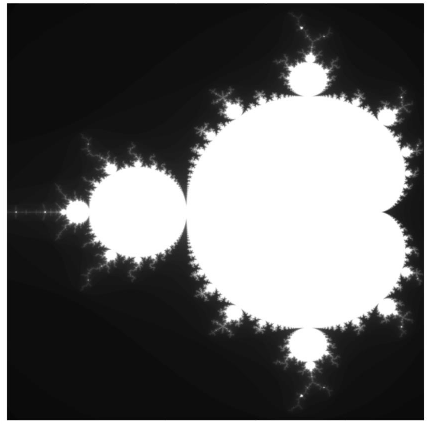
\includegraphics[width=3.5cm]{images/mandelbrot}
  \end{center}
  
\end{frame}

%%%%%%%%%%%%%%%%%%%%%%%%%%%%%%%%%%%%%%%%%%%%%%%%%%%%%%%%%%%%%%%%%%%%%%%% 
%%%%%%%%%%%%%%%%%%%%%%%%%%%%%%%%%%%%%%%%%%%%%%%%%%%%%%%%%%%%%%%%%%%%%%%% 
\begin{frame}[fragile=singleslide]
  \frametitle{Hands-On 3 : Mandelbrot set}

  {\Large \textcolor{darkgreen}{\textbf{Proposed activity:}}\\ \textbf{refactor this computing loop into a C++ Kokkos functor class}}
  \begin{itemize}
  \item See \textcolor{blue}{kokkos basic version} from \texttt{code/handson/3/mandelbrot\_kokkos/kokkos\_basic} (already a bit refactored to ease the job)
  \end{itemize}
  %
  \begin{enumerate}
  \item we added a file \textcolor{blue}{\texttt{kokkos\_shared.h}}: \texttt{std::vector} replaced by a \texttt{Kokkos::View}
  \item \textcolor{orange}{\textbf{TODO:}} fill TODOs in \texttt{mandelbrot.h} containing the definition of the c++ mandelbrot kokkos functor.\\
    \textbf{Notice:} the global constants have disappeared, they are now part of the functor context.
  \item \textcolor{orange}{\textbf{TODO:}} refactor \texttt{main.cpp} (change the TODO)
    \begin{itemize}
    \item Modify data allocation (from \texttt{std::vector} to \texttt{Kokkos::View}); we have now arrays: \texttt{image} and \texttt{imageHost} (mirror)
    \item Copy back results from device to host.
    \end{itemize}
  \end{enumerate}
  
\end{frame}

%%%%%%%%%%%%%%%%%%%%%%%%%%%%%%%%%%%%%%%%%%%%%%%%%%%%%%%%%%%%%%%%%%%%%%%% 
%%%%%%%%%%%%%%%%%%%%%%%%%%%%%%%%%%%%%%%%%%%%%%%%%%%%%%%%%%%%%%%%%%%%%%%% 
\begin{frame}[fragile=singleslide]
  \frametitle{Hands-On 3 : Mandelbrot set}

  \begin{itemize}
    % \item The provided \texttt{Makefile} is designed to be used with kokkos environment from a modulefile
  \item Use code from directory \texttt{code/handson/3}; it is designed to work with cmake
  \item Build the \textcolor{blue}{\texttt{kokkos\_basic}} version
  \item \textcolor{violet}{\textbf{OpenMP}}
    \begin{itemize}
    %\item \texttt{module use /pwrwork/workshops/patc-201701/kokkos/modulefiles}
    %\item \texttt{module load kokkos/openmp\_gnu485\_dev}
    \item \texttt{mkdir build\_openmp; cd build\_openmp}
    \item \texttt{cmake -DKOKKOS\_ENABLE\_OPENMP=ON ..; make}
    \end{itemize}
  \item \textcolor{violet}{\textbf{Cuda}}
    \begin{itemize}
    %\item \texttt{module use /pwrwork/workshops/patc-201701/kokkos/modulefiles}
    %\item \texttt{module load cuda/8.0 kokkos/cuda80\_gnu485\_dev\_k80}
    \item \texttt{mkdir build\_cuda; cd build\_cuda\_kepler37}
    \item \texttt{export CXX=/full/path/to/nvcc\_wrapper}
    \item \texttt{cmake -DKOKKOS\_ENABLE\_CUDA=ON -DKOKKOS\_ARCH=Kepler37 ..}
    \item you also add \texttt{-DKOKKOS\_ENABLE\_CUDA\_LAMBDA=ON}; you can also build again for architecture Pascal60
    \item \texttt{make}
    \end{itemize}
  \item \textbf{Compare performance} for a large Mandelbrot set $8192\times 8192$ : OpenMP versus Cuda
  \end{itemize}

\end{frame}
  
%%%%%%%%%%%%%%%%%%%%%%%%%%%%%%%%%%%%%%%%%%%%%%%%%%%%%%%%%%%%%%%%%%%%%%%% 
%%%%%%%%%%%%%%%%%%%%%%%%%%%%%%%%%%%%%%%%%%%%%%%%%%%%%%%%%%%%%%%%%%%%%%%% 
\begin{frame}[fragile=singleslide]
  \frametitle{Hands-On 3 : Mandelbrot set}

  \begin{itemize}
  \item {\bf Additionnal:} revisit this simple example using a \textcolor{blue}{\bf multidimensional range policy} to launch the Mandelbrot functor:
  \end{itemize}
  \begin{minted}{c++}
    Kokkos::Experimental::MDRangePolicy< Kokkos::Experimental::Rank<2> ,
                                         Kokkos::IndexType<int> >;
  \end{minted}
  \begin{itemize}
  \item \textcolor{orange}{\textbf{TODO:}} fill TODOs in \texttt{mandelbrot.h} and \texttt{main.cpp} in directory \texttt{mandelbrot\_kokkos/kokkos\_mdrange}
  \item \textcolor{red}{\bf This way avoids the use of linearized indexes.}
  \end{itemize}

\end{frame}

%%%%%%%%%%%%%%%%%%%%%%%%%%%%%%%%%%%%%%%%%%%%%%%%%%%%%%%%%%%%%%%%%%%%%%%% 
%%%%%%%%%%%%%%%%%%%%%%%%%%%%%%%%%%%%%%%%%%%%%%%%%%%%%%%%%%%%%%%%%%%%%%%% 
\begin{frame}[fragile=singleslide]
  \frametitle{Hands-On 3 : Mandelbrot set}

  \begin{itemize}
  \item Pipelined version of Mandelbrot is not currently fully functional; it requires a small patch applied to \texttt{Kokkos} for \texttt{cudaStreams};\\
    see \myurl{https://github.com/kokkos/kokkos/issues/532}
  \item Understand what is pipelined version of Mandelbrot see:
    {\scriptsize \myurl{http://on-demand.gputechconf.com/gtc/2015/webinar/openacc-course/advanced-openacc-techniques.pdf}}\\
    It basically consists in overlapping GPU computations with CPU/GPU memory transfert.
  \item See explanations given during training
  \end{itemize}

\end{frame}


\subsection{Stencil / Finite Difference}
% hands-on 4 : 2D Kokkos::View
%%%%%%%%%%%%%%%%%%%%%%%%%%%%%%%%%%%%%%%%%%%%%%%%%%%%%%%%%%%%%%%%%%%%%%%% 
%%%%%%%%%%%%%%%%%%%%%%%%%%%%%%%%%%%%%%%%%%%%%%%%%%%%%%%%%%%%%%%%%%%%%%%% 
\begin{frame}[fragile=singleslide]
  \frametitle{Hands-On 4 : Finite Difference / Stencil}

  \hypertarget{handson4}{}

  \begin{itemize}
  \item Illustrate the use of 2D \texttt{Kokkos::View}
  \end{itemize}
  
\end{frame}

\subsection{Laplace solver}
% hands-on 5 : pure Kokkos versus Kokkos + MPI + hwloc
%%%%%%%%%%%%%%%%%%%%%%%%%%%%%%%%%%%%%%%%%%%%%%%%%%%%%%%%%%%%%%%%%%%%%%%% 
%%%%%%%%%%%%%%%%%%%%%%%%%%%%%%%%%%%%%%%%%%%%%%%%%%%%%%%%%%%%%%%%%%%%%%%% 
\begin{frame}
  \frametitle{Hands-On 5 : Laplace solver with KOKKOS + MPI}

  Slightly adapted from Nvidia's OpenACC exercise:\\
  \myhref{https://github.com/NVIDIA-OpenACC-Course/nvidia-advanced-openacc-course-sources}{nvidia-advanced-openacc-course-sources}

  We will use code from \myurl{code/exercises/laplace_kokkos}, 4 different versions of the 2D Laplace solver:
  \begin{itemize}
  \item serial (no kokkos)
  \item kokkos with 1D viewd (linearized index)
  \item kokkos\_v2 with 2D views
  \item kokkos\_mpi with MPI+CUDA and hwloc
  \end{itemize}
  
\end{frame}


\subsection{MiniApp - Kokkos lambda}
% hands-on 6
%%%%%%%%%%%%%%%%%%%%%%%%%%%%%%%%%%%%%%%%%%%%%%%%%%%%%%%%%%%%%%%%%%%%%%%% 
%%%%%%%%%%%%%%%%%%%%%%%%%%%%%%%%%%%%%%%%%%%%%%%%%%%%%%%%%%%%%%%%%%%%%%%% 
\begin{frame}
  \frametitle{Hands-On 7 - Reaction-Diffusion Fisher equation (1)}

  \begin{itemize}
  \item \textcolor{red}{\textbf{SETUP}}: we will use git to download this miniApp code designed at \myhref{http://www.cscs.ch/index.html}{CSCS} for HPC teaching purpose.
    % See file \myurl{code/miniapps/SummerSchool2016/readme.md} to know how
    % to download the code 
    \begin{itemize}
    \item \texttt{cd \$HOME/patc\_kokkos/code/miniapps/SummerSchool2016}
    \item \texttt{git clone https://github.com/pkestene/SummerSchool2016.git}
    \item \texttt{cd Summerschool2016; git checkout kokkos}
    \end{itemize}
  \item \textbf{This material contains multiple versions} of a \textcolor{violet}{\textbf{Reaction-Diffusion PDE solver (Fisher equation used e.g. in popualtion dynamics)}}. We will contribute two Kokkos versions of this solver.
    $$ \frac{\partial s}{\partial t} = D \left( \frac{\partial^2 s}{\partial x^2} + \frac{\partial^2 s}{\partial y^2} \right) + R s (1-s) = 0$$
  \end{itemize}
  
\end{frame}

%%%%%%%%%%%%%%%%%%%%%%%%%%%%%%%%%%%%%%%%%%%%%%%%%%%%%%%%%%%%%%%%%%%%%%%% 
%%%%%%%%%%%%%%%%%%%%%%%%%%%%%%%%%%%%%%%%%%%%%%%%%%%%%%%%%%%%%%%%%%%%%%%% 
\begin{frame}
  \frametitle{Hands-On 7 - Reaction-Diffusion Fisher equation (2)}

  \begin{enumerate}
  \item \textbf{Explore/Read slides about the Fisher solver:}\\
    {\footnotesize \texttt{\$HOME/patc\_kokkos/code/miniapps/SummerSchool2016/miniapp/kokkos/serial/miniapp.pdf}}
    \begin{itemize}
    \item Explore the \textcolor{red}{serial} version of the Fisher solver.
    \end{itemize}
  \item These \textbf{Kokkos exercises} are routed to use the \textcolor{darkgreen}{\textbf{modulefiles}}:
    \begin{itemize}
    \item \texttt{module use /pwrwork/workshops/patc-201701/kokkos/modulefiles}
    \item \texttt{module load kokkos/openmp\_gnu485\_dev}
    \item \texttt{make}
    \end{itemize}
  \item \textcolor{blue}{\textbf{Kokkos version 1}} / Exercice with \texttt{KOKKOS\_LAMBDA} / Already pre-filled, some TODOs
    \begin{itemize}
    \item Open and read file \texttt{miniapp/kokkos/cxx/readme.txt}
    \item Fill the TODO with Kokkos LAMBDA kernels
    \end{itemize}
  \item \textcolor{blue}{\textbf{Kokkos version 2}} : already done
    \begin{itemize}
    \item The main difference between version 1 and 2 is how the c++ class \texttt{DataWareHouse} is designed
    \item Just build and compare performance with version 1, with Kokkos device OpenMP(Power8) and then Cuda
    \end{itemize}
  \end{enumerate}
\end{frame}


\subsection{MiniApp - Performance}
% hands-on 7
%%%%%%%%%%%%%%%%%%%%%%%%%%%%%%%%%%%%%%%%%%%%%%%%%%%%%%%%%%%%%%%%%%%%%%%% 
%%%%%%%%%%%%%%%%%%%%%%%%%%%%%%%%%%%%%%%%%%%%%%%%%%%%%%%%%%%%%%%%%%%%%%%% 
\begin{frame}[fragile=singleslide]
  \frametitle{Hands-On 8 : Euler equation solver}

  \hypertarget{handson8}{}
  \begin{itemize}
  \item Original serial code: \texttt{\$HOME/patc\_kokkos/code/miniapps/euler2d\_serial}
  \item See additionnal slides in source directory about CFD numerics
  \item \textcolor{red}{\bf Activity 1: Porting code to kokkos:} the serial version has been partially ported to kokkos; fill the TODOs to complete.
  \item \textcolor{darkgreen}{\bf Activity 2: Build / run / mesure performance} of the kokkos solution (directory \texttt{euler2d\_kokkos\_solution}). Try to plot the OpenMP weak scaling on Power8.
  \item {\bf How much faster is the GPU version (Pascal P100) versus the Power8 ?}
  \end{itemize}
  
  \begin{center}
    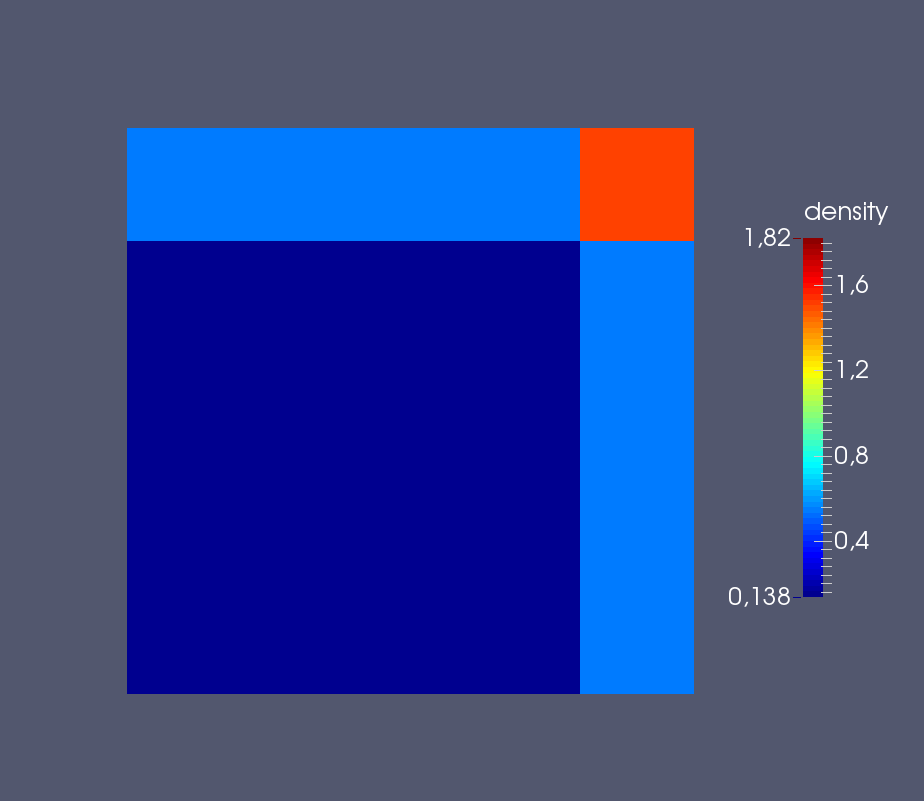
\includegraphics[height=3.0cm]{../euler/images/riemann/riemann_1}
    \hspace{0.1cm}
    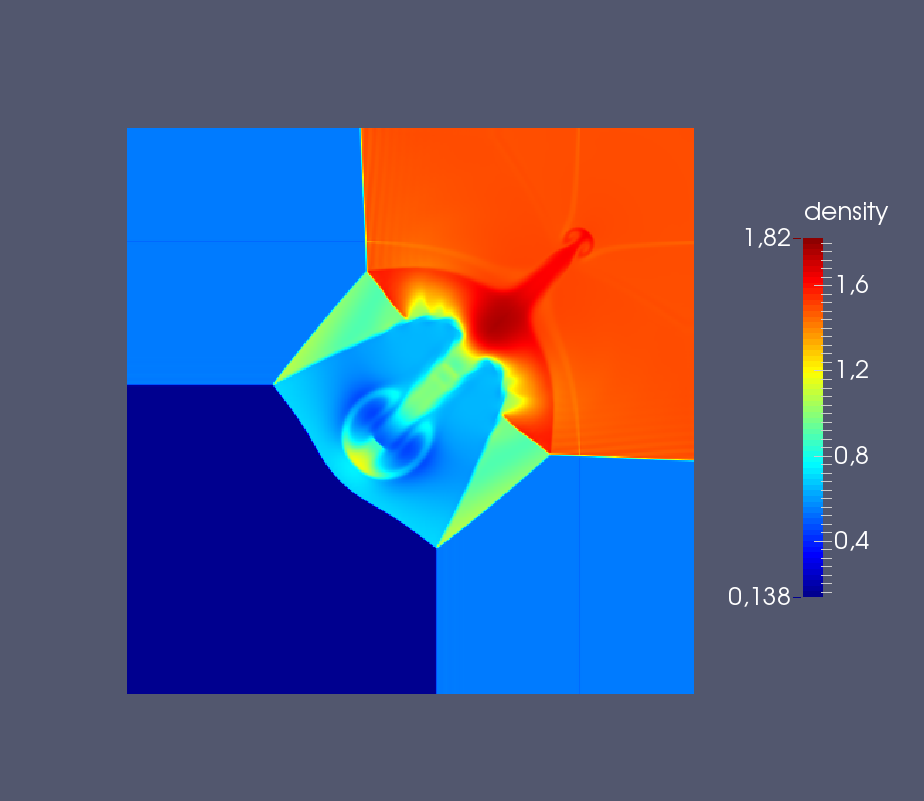
\includegraphics[height=3.0cm]{../euler/images/riemann/riemann_2}
  \end{center}


\end{frame}


\section{Additionnal Kokkos material}

\subsection{Use an installed version of Kokkos}
%%%%%%%%%%%%%%%%%%%%%%%%%%%%%%%%%%%%%%%%%%%%%%%%%%%%%%%%%%%%%%%%%%%%%%%% 
%%%%%%%%%%%%%%%%%%%%%%%%%%%%%%%%%%%%%%%%%%%%%%%%%%%%%%%%%%%%%%%%%%%%%%%% 
\begin{frame}[fragile=singleslide]
  \frametitle{Using an installed Kokkos (deprecated)}

  {\large \bf I strongly recommend starting using cmake to integrate kokkos in your application.} But just in case, you're still interested:
  \begin{itemize}
  \item As you will surely \textcolor{red}{\textbf{use multiple versions}} of Kokkos (OpenMP, Cuda, ...), with/without Lambda, UVM, different compilers, etc ... it will be very usefull to use some \textbf{modulefiles}.
  \item A \textcolor{blue}{\textbf{module environment}} is not a tool specific to a super-computer, it can be used on a \textbf{Desktop/Laptop} to configure an execution environment.\\
    e.g. \textcolor{blue}{\texttt{sudo apt-get install environment-modules}} (Debian/Ubuntu)
  \item \textcolor{blue}{What is a modulefiles ?}
    A simple way to set env variables to ease the use of a given software package.
  \item You will find some examples modulefiles for Kokkos in \texttt{/pwrwork/workshops/patc-201701/kokkos/modulefiles/kokkos} you can easily adapt to your own platform.
  \end{itemize}

\end{frame}

%%%%%%%%%%%%%%%%%%%%%%%%%%%%%%%%%%%%%%%%%%%%%%%%%%%%%%%%%%%%%%%%%%%%%%%% 
%%%%%%%%%%%%%%%%%%%%%%%%%%%%%%%%%%%%%%%%%%%%%%%%%%%%%%%%%%%%%%%%%%%%%%%% 
\begin{frame}[fragile=singleslide]
  \frametitle{Using an installed Kokkos (2)}

  \begin{itemize}
  \item A simple modulefiles for Kokkos should at minimum set variable \textcolor{blue}{\texttt{KOKKOS\_PATH}} pointing to the installed directory (the one which contains \textcolor{blue}{\texttt{Makefile.kokkos}}
  \item {\bf How to use Kokkos modulefiles on \textcolor{blue}{your own machine} ?} Just use the following: 
    {\small
      \begin{minted}{bash}
        # Assuming you placed the module file in
        # /somewhere_on_your_machince/modulefiles
        module use /somewhere_on_your_machince/modulefiles
        
        # e.g. load Kokkos for GPU
        module load kokkos/cuda80_gnu485_dev_k80
      \end{minted}
    }
  \item {\bf How to use Kokkos modulefiles on \textcolor{red}{ouessant} ?} Just use the following:
    {\small
      \begin{minted}{bash}
        # Assuming you placed the module file in
        # /somewhere_on_your_machince/modulefiles
        module use /pwrwork/workshops/patc-201701/kokkos/modulefiles
        # e.g. load Kokkos for GPU
        module load kokkos/cuda80_gnu485_dev_k80
      \end{minted}
    }
  \end{itemize}

\end{frame}


\subsection{Use Kokkos from Trilinos}
%%%%%%%%%%%%%%%%%%%%%%%%%%%%%%%%%%%%%%%%%%%%%%%%%%%%%%%%%%%%%%%%%%%%%%%% 
%%%%%%%%%%%%%%%%%%%%%%%%%%%%%%%%%%%%%%%%%%%%%%%%%%%%%%%%%%%%%%%%%%%%%%%% 
\begin{frame}
  \frametitle{About Kokkos in Trilinos}

  \begin{itemize}
  \item \myhref{https://github.com/kokkos/kokkos}{kokkos} is originally a subpackage of \myhref{https://trilinos.org/}{trilinos} (application framework for solving problems requiring parallel large distributed linear algebra solvers).
  \item Kokkos is the performance portable layer, to allow running Trilinos as efficiently as possible on multiple architectures.
  \item Kokkos can be build independently from Trilinos and used in other applications
  \end{itemize}

  \begin{center}
    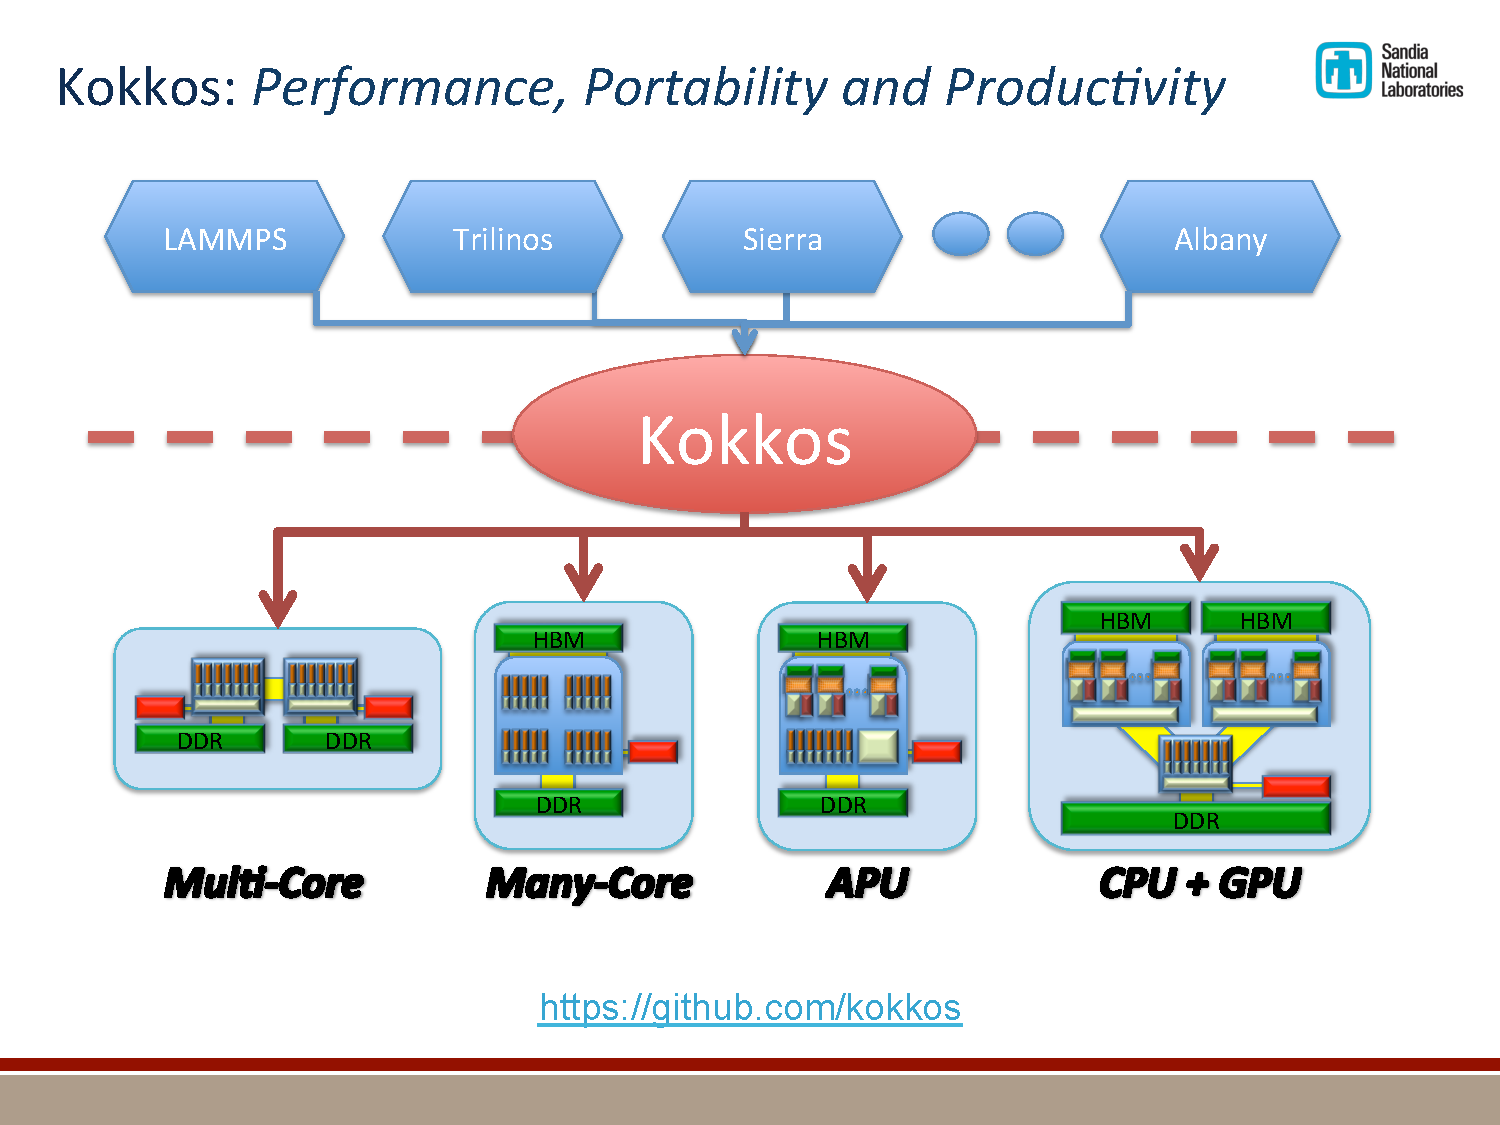
\includegraphics[width=6cm]{images/Kokkos-Multi-CoE_slide2}
  \end{center}
  
\end{frame}

%%%%%%%%%%%%%%%%%%%%%%%%%%%%%%%%%%%%%%%%%%%%%%%%%%%%%%%%%%%%%%%%%%%%%%%% 
%%%%%%%%%%%%%%%%%%%%%%%%%%%%%%%%%%%%%%%%%%%%%%%%%%%%%%%%%%%%%%%%%%%%%%%% 
\begin{frame}
  \frametitle{About Kokkos in Trilinos}

  \begin{itemize}
  \item \textbf{Build a minimal featured Trilinos with Kokkos for GPU activated} : \textcolor{red}{Tpetra + kokkos + Cuda}
    \begin{enumerate}
    \item \textbf{Example config plateform:} Ubuntu 16.04 + openmpi + cuda 8.0\\
      compiler is gcc 5.4.0
    \item \textbf{Get Trilinos sources:}\\
      \texttt{git clone https://github.com/trilinos/Trilinos.git;} \texttt{cd Trilinos; git checkout develop}
    \item \textbf{CMake configuration script:} Use the provided configuration file \texttt{configure\_tpetra\_kokkos\_cuda\_nvcc\_wrapper.sh} located in the provided archive (\texttt{doc/trilinos})\\
      this script needs slights changes (var \texttt{OMPI\_CXX} and install prefix)\\
      this script must be run in a build directory (not directly in trilinos sources).\\
      this config will build kokkos with unit tests and examples.
    \item \textbf{Build:} \texttt{make -j; make install}
    \item \textbf{Build a sample project.}
    \end{enumerate}
  \end{itemize}

\end{frame}

%%%%%%%%%%%%%%%%%%%%%%%%%%%%%%%%%%%%%%%%%%%%%%%%%%%%%%%%%%%%%%%%%%%%%%%% 
%%%%%%%%%%%%%%%%%%%%%%%%%%%%%%%%%%%%%%%%%%%%%%%%%%%%%%%%%%%%%%%%%%%%%%%% 
\begin{frame}
  \frametitle{Trilinos/Tpetra example project}

  \begin{itemize}
  \item Directory \texttt{doc/trilinos/tpetra\_example} contains a minimal example application for trilinos/tpetra. You just need to set env variable \texttt{TRILINOS\_PATH} to install directory.
  \end{itemize}
  
\end{frame}


\end{document}
